\documentclass[11pt]{article}
\usepackage[margin=1.15in]{geometry}
\usepackage{xcolor}
\usepackage{amsmath,amssymb,amsthm,mathtools,booktabs,graphicx,enumitem,hyperref,cleveref,microtype,xurl}
\graphicspath{{../figures/}}
\hypersetup{colorlinks=true,linkcolor=blue!50!black,citecolor=blue!50!black,urlcolor=blue!50!black,
 pdftitle={Arithmetic Transport and Dimensional Obstructions in UNNS Occurrence Geometry},
 pdfauthor={UNNS Research Collective},
 pdfsubject={Manuscript I of the GEO-HD-1 programme: lattice transport of occurrence geometry},
 pdfkeywords={occurrence set; relation lattice; Graver basis; zonotopal tiling; transport; dimensional obstruction}}
\theoremstyle{plain}
\newtheorem{theorem}{Theorem}[section]
\newtheorem{lemma}[theorem]{Lemma}
\newtheorem{proposition}[theorem]{Proposition}
\newtheorem{corollary}[theorem]{Corollary}
\theoremstyle{definition}
\newtheorem{definition}[theorem]{Definition}
\newtheorem{example}[theorem]{Example}
\newtheorem{problem}[theorem]{Problem}
\theoremstyle{remark}
\newtheorem{remark}[theorem]{Remark}
\crefname{theorem}{Theorem}{Theorems}\crefname{lemma}{Lemma}{Lemmas}\crefname{proposition}{Proposition}{Propositions}
\crefname{corollary}{Corollary}{Corollaries}\crefname{definition}{Definition}{Definitions}\crefname{example}{Example}{Examples}
\crefname{section}{Section}{Sections}\crefname{figure}{Figure}{Figures}\Crefname{figure}{Figure}{Figures}
% ---- notation
\newcommand{\Z}{\mathbb Z}\newcommand{\R}{\mathbb R}\newcommand{\Q}{\mathbb Q}\newcommand{\N}{\mathbb N}
\newcommand{\Gr}{\operatorname{Gr}}\newcommand{\Kabs}{K_{\mathrm{abs}}}\newcommand{\Kemb}{K_{\mathrm{emb}}}
\newcommand{\cm}{\preceq}   % conformal order
\newcommand{\Cmap}{\mathcal C}
\newcommand{\Pcal}{\mathcal P}
\newcommand{\Pil}{\Pi}
\newcommand{\supp}{\operatorname{supp}}
\newcommand{\ord}{\operatorname{ord}}
\newcommand{\conv}{\operatorname{conv}}
\newcommand{\rk}{\operatorname{rank}}
\newcommand{\Even}{E}
% provenance line: \prov{uid}{source id}{status}{treatment}
\newwrite\provw
\immediate\openout\provw=\jobname.prov
\newcommand{\provrow}[6]{\texttt{#1} & \texttt{#2} & #3 & #4 & #5 & #6}
\newcommand{\prov}[4]{\par\smallskip\noindent{\footnotesize\textit{Source record:} \texttt{#2} (\texttt{#1}); status \textsc{#3}; treatment \textsc{#4}.}\par
 \immediate\write\provw{\string\provrow{#1}{#2}{#3}{#4}{\thesection}{\thetheorem}}}
\title{Arithmetic Transport and Dimensional Obstructions\\ in UNNS Occurrence Geometry}
\author{UNNS Research Collective\\[2pt]\small Manuscript I of the programme \emph{GEO-HD-1} --- version 0.4}
\date{2 November 2026}
\setlength{\emergencystretch}{2em}
\renewcommand{\topfraction}{0.9}\renewcommand{\bottomfraction}{0.8}\renewcommand{\textfraction}{0.08}\renewcommand{\floatpagefraction}{0.6}\setcounter{topnumber}{3}\setcounter{totalnumber}{4}
\begin{document}
\maketitle
\begin{abstract}
For a reduced rational $x=a/b$ let $D(x)$ be the set of integers $d\ge2$ with $d^2\mid a$ and $d\equiv1\pmod b$. In exponent coordinates over the primes whose squares divide $a$, $D(x)$ is the set of nonzero points of a box lying in a lattice $\Lambda_b$ defined by one congruence. The Graver moves of $\Lambda_b$ span parallelotopes, and their union $U$ is the realised geometry of the state. When the denominator changes the lattice changes, and we ask what survives; we call this question \emph{transport}.

We separate three notions of survival (vertices, cells of the abstract cell complex, and containment of the realised union) and prove exact criteria for each. In the plane the realised union is monotone under every inclusion of relation lattices, for every box (Theorem~\ref{thm:planar}). In dimension three this fails: in infinite families closed under diagonal dilation, including targets with no free coordinate, and for a target that is split in no coordinate, the union of the source is not contained in the union of the target (Theorem~\ref{thm:C1} and Proposition~\ref{prop:C3}). The failure is carried by cells that touch all coordinate hyperplanes, which we call hard cells. When the target splits along one coordinate, an exact slab criterion decides containment; it replaces the closed-height criterion of an earlier release (Theorem~\ref{thm:slab-ii}). Statements proved by finite exact computation are kept separate, with their scopes, from the theorems.
\end{abstract}
\tableofcontents
\section{Introduction}\label{sec:intro}
Each reduced rational $x=a/b$ has an occurrence set $D(x)=\{d\ge2: d^2\mid a,\ d\equiv1 \pmod b\}$. Writing the divisors in exponent coordinates over the primes whose squares divide $a$ identifies $D(x)$ with the nonzero points of a box intersected with a lattice $\Lambda_b$ of exponent vectors defined by one congruence (\cref{prop:fibre}). This finite set, with its Graver moves, parallelotopes and their union, is the geometry studied in the GEO-I releases of the UNNS programme~\cite{GEOI}: its Graver moves, the parallelotopes they span, and the union of those parallelotopes.

The question of this manuscript is what happens when the arithmetic moves. Under the collective map $x\mapsto\Cmap(x)=x+L^2/G$, with $L=\operatorname{lcm}D(x)$ and $G=\gcd\{d-1:d\in D(x)\}$ (the rational dynamics FIELD-I of the programme~\cite{FoundII}), the occurrence set can only grow, $D(x)\subseteq D(\Cmap(x))$, but the lattice and its Graver set change, and geometric structure that existed before need not exist afterwards, nor conversely. We call the study of such comparisons \emph{transport}. The manuscript treats it for explicitly defined source and target lattices and a fixed box; the evolution of whole orbits is the subject of a later manuscript.

\paragraph{Three objects.} For a lattice $\Lambda$ and box $Q$ we use three objects that are \emph{not} interchangeable: the abstract complex $\Kabs(\Lambda,Q)$ of cells, the realised union $U(\Lambda,Q)\subset\R^k$ of the corresponding closed parallelotopes, and, when the cells meet only in common faces, the embedded subdivision $\Kemb$. Every statement below names the object it concerns.

\paragraph{Results.}
\begin{enumerate}[label=(\Roman*)]
\item \emph{Exact criteria (Sections~\ref{sec:lattice}--\ref{sec:cells}).} Inclusion of relation lattices is decided from finitely many group data (\cref{thm:P2T1}). A cell of the source survives in the abstract target complex exactly when its vertices lie in the target fibre and its generators are Graver moves of the target (\cref{thm:cell-transport}); hence no cell of dimension larger than the rank of the common Graver moves survives. For the three-stage orbit $P^4/3\to2P^4/3\to P^4$ all positive-dimensional cells are lost for every number $k\ge2$ of primes (\cref{cor:threestage}), although the occurrence set strictly grows.
\item \emph{Abstract loss is not geometric loss (\cref{sec:realised}).} Every abstractly lost edge of that orbit still lies in the target union (\cref{thm:E28}), while some two-dimensional cells leave it (\cref{prop:E29}); four plausible monotonicity laws are refuted by exact witnesses.
\item \emph{Rectangular targets and the corner cube (\cref{sec:corner}).} For a target lattice $\bigoplus o_i\Z$ the uncovered region is exactly an open corner cube $O$; edges never meet it in any dimension, so the union is preserved for $k=2$ (\cref{thm:corner}), while for $k=3$ the failure is governed by two-dimensional cells and, for the even-sum source, occurs exactly when the scaled box has a side $\ge2$ (\cref{thm:evensum}).
\item \emph{Planar monotonicity (\cref{sec:planar}).} For every inclusion $\Lambda\subseteq\Lambda'$ of full-rank lattices of $\Z^2$ and every box, $U(\Lambda,Q)\subseteq U(\Lambda',Q)$ (\cref{thm:planar}). The proof isolates \emph{hard} cells, those that touch every coordinate hyperplane, and shows that in the plane their geometry forces coverage.
\item \emph{Dimensional obstruction (\cref{sec:obstruction}).} Containment fails in dimension three, in infinite families closed under diagonal dilation, with a target having no free coordinate (\cref{thm:C1}); and also for a target, the body-centred lattice, that is not split in any coordinate (\cref{prop:C3}, finite-exact).
\item \emph{Slab criterion (\cref{sec:slab}).} For a target that splits along one coordinate with period $k$, the union is an explicit stack of planar unions, and containment of a cell is a planar condition. The criterion as first published (closed height) is false; we prove and use the corrected form (\cref{thm:slab-ii}).
\end{enumerate}

\paragraph{What is not claimed.} Statements checked only by finite exact computation are labelled FINITE-EXACT and carry their domain. Nothing is asserted about arbitrary lattices outside the stated families, and no planar theorem is extended to dimension three. Several results are elementary; no priority claim is made. The classification of non-split three-dimensional targets that preserve the union is open (\cref{sec:open}).

\paragraph{Relation to earlier work.} The relation lattices, Graver cells and planar stabilisation theory are inherited from GEO-I~\cite{GEOI} and the Foundations volumes~\cite{FoundI,FoundII,RefColl} and are cited with their hypotheses; the planar stabilisation theorem G12-T8 is used only as a cited prerequisite (\cref{sec:g12}). Throughout, \texttt{CW-nnnn} denotes the row of the consolidated theorem crosswalk and the second identifier is the source theorem name; \cref{app:map} lists all of them.

\paragraph{Reading guide to the figures.} The geometric arguments are illustrated where they are made. \Cref{fig:objects} fixes the three objects; \cref{fig:equalfibres,fig:threestage,fig:planar} illustrate the transport of lattices and of abstract cells; \cref{fig:dim,fig:corner} the corner cube; \cref{fig:lost} the difference between abstract loss and containment; \cref{fig:planarproof} the planar theorem; \cref{fig:noncontain,fig:dilation,fig:bcc} the three-dimensional obstructions; \cref{fig:slab,fig:strict} the slab criterion; \cref{fig:hardcell,fig:f110} hard cells and the coupled specimen. Each caption states whether the picture is an \emph{exact computation} (coordinates produced and checked in exact rational arithmetic by \texttt{scripts/figs\_*.py}; the data are in \texttt{results/FIGURE\_DATA.json}), a \emph{theorem-level construction} (exact coordinates of the construction in a proof) or a \emph{schematic}. Colours: source structures blue, targets teal, surviving relations green, lost relations red, uncovered regions light orange, witnesses magenta stars; every distinction is also carried by line style, hatching or marker shape.

\section{Setting and notation}\label{sec:setting}

\subsection{Fibres of occurrence sets}
A \emph{state} is a positive rational $x=a/b$ in lowest terms. Its occurrence set is $D(x)=\{d\ge2: d^2\mid a,\ d\equiv1\ (\mathrm{mod}\ b)\}$ (Foundations Vol.~I, Thm.~1.2~\cite{FoundI}). Let $\Pcal=\{p_1<\dots<p_k\}$ be the primes with $p_i^2\mid a$, $q_i=\lfloor v_{p_i}(a)/2\rfloor\ge1$, and $Q=\prod_{i}[0,q_i]$ the \emph{box}. For $\alpha\in\Z^k$ put $\chi_b(\alpha)=\prod_i p_i^{\alpha_i}\bmod b$ (negative exponents through inverses; $\gcd(p_i,b)=1$ because $\gcd(a,b)=1$) and
\[
\Lambda_b=\ker\chi_b\subseteq\Z^k,\qquad F(\Lambda,Q)=(\Lambda\cap Q)\setminus\{0\}.
\]
\begin{proposition}[fibre]\label{prop:fibre}
The map $\alpha\mapsto\prod p_i^{\alpha_i}$ is a bijection $F(\Lambda_b,Q)\to D(x)$. The index is $[\Z^k:\Lambda_b]=|H_b|$ with $H_b=\langle p_1,\dots,p_k\rangle\le(\Z/b)^\times$.
\end{proposition}
\begin{proof}
If $d^2\mid a$ then every prime factor $p$ of $d$ has $p^2\mid a$, so $d=\prod p_i^{\alpha_i}$ with $0\le\alpha_i\le q_i$; this exponent vector is unique, and $d\equiv1\pmod b$ iff $\chi_b(\alpha)=1$. The vector $\alpha=0$ gives $d=1\notin D(x)$. The map $\chi_b:\Z^k\to H_b$ is onto with kernel $\Lambda_b$. \qedhere
\end{proof}
For $b=1$ we have $\Lambda_1=\Z^k$. A lattice here always means a full-rank sublattice of $\Z^k$ (finite index); this holds for every $\Lambda_b$.

\subsection{Moves, cells and the three objects}
\begin{definition}[conformal order, Graver set]
For $v,w\in\Z^k$ write $w\cm v$ if $w_iv_i\ge0$ and $|w_i|\le|v_i|$ for all $i$. For a lattice $\Lambda$, $\Gr(\Lambda)$ is the set of $\cm$-minimal nonzero elements of $\Lambda$ (the \emph{Graver set}); it is symmetric under $v\mapsto-v$ (Graver~\cite{Graver1975}; see also \cite{Sturmfels1996,DLHK2013}). For $q\in\Z_{>0}^k$ the \emph{region Graver set} $\Gr_q(\Lambda)$ is the set of $\cm$-minimal nonzero elements of $\Lambda\cap[-q,q]$.
\end{definition}
\begin{definition}[cell]\label{def:cell}
Let $g_1,\dots,g_j\in\Gr_q(\Lambda)$ be linearly independent and $u\in\Z^k$. The parallelotope $\Pil(u;g_1,\dots,g_j)=u+\sum_i[0,1]g_i$ is a \emph{$j$-cell of $(\Lambda,Q)$} if all its $2^j$ corners lie in $F(\Lambda,Q)$. (A $0$-cell is a point of $F$.) The \emph{abstract complex} $\Kabs(\Lambda,Q)$ is the set of all cells, a cell being identified with its vertex set (\cref{lem:intrinsic}); it is closed under taking faces. The \emph{realised union} is $U(\Lambda,Q)=\bigcup$ of the closed cells. The \emph{origin-allowed union} $U^0(\Lambda,Q)$ is defined in the same way with the corners allowed to be $0$.
\end{definition}
The origin is excluded because $\alpha=0$ corresponds to $d=1\notin D(x)$. This single exclusion is the source of every phenomenon in this manuscript. A third object, the \emph{embedded subdivision} $\Kemb$, exists only when any two closed cells meet in a common face; it is never needed below and when a statement is about $\Kabs$, $U$ or $\Kemb$ it says so. Boundaries of cells in $\Kabs$ are $\partial\Pil(u;g_1..g_j)=\sum_i(-1)^{i-1}[\Pil(u+g_i;\widehat{g_i})-\Pil(u;\widehat{g_i})]$; $\partial\partial=0$.

\begin{lemma}[cells are intrinsic]\label{lem:intrinsic}
Order $\Z^k$ lexicographically. A cell $c$ with vertex set $V(c)$ has its lexicographically smallest vertex $m(c)$ as a base point and the set $\mathrm{Gen}(c)$ of its generators, taken lexicographically positive, equals the set of edge vectors of $\conv V(c)$ at $m(c)$. In particular $V(c)$ determines $c$ and $\mathrm{Gen}(c)$.
\end{lemma}
\begin{proof}
$\conv V(c)=\Pil(u;g_1..g_j)$ is a $j$-dimensional parallelotope; its vertices are $u+\sum_{i\in S}g_i$. The lexicographic order is translation invariant, so the smallest vertex is $u+\sum_{g_i<0}g_i$, and the edges at that vertex of the parallelotope are along $\pm g_i$ leaving in the lexicographically positive direction. Edges of $\conv V(c)$ depend only on the convex body, hence only on $V(c)$. \qedhere
\end{proof}
Remark: since $\Gr_q(\Lambda)=-\Gr_q(\Lambda)$, ``$\mathrm{Gen}(c)\subseteq\Gr_q(\Lambda)$'' does not depend on orientations.
\begin{figure}[tbp]\centering
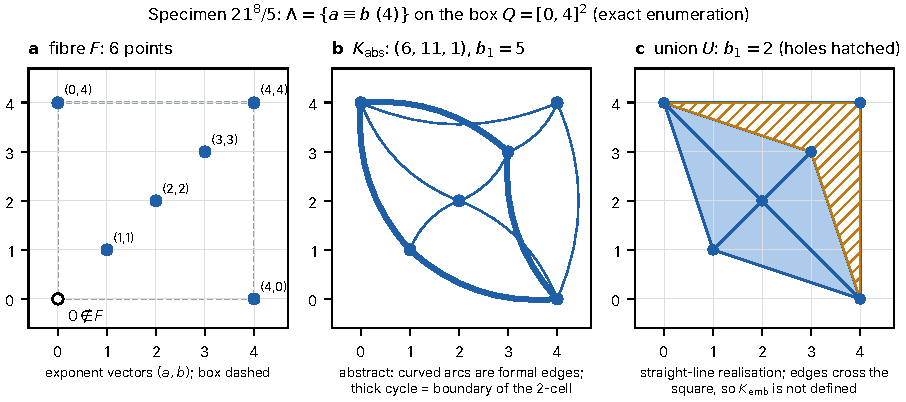
\includegraphics[width=0.98\textwidth]{fig01_three_objects}
\caption{The three objects for the specimen $21^8/5$ ($\Lambda=\{a\equiv b\ (4)\}$, $Q=[0,4]^2$; \emph{exact computation}). (a)~The fibre $F(\Lambda,Q)$: six points, the origin being excluded. (b)~The abstract complex $\Kabs$: f-vector $(6,11,1)$, Betti numbers $(1,5,0)$; edges are drawn as arcs to stress that they are formal incidences, and the thick cycle bounds the single $2$-cell. (c)~The realised union $U$ of the closed cells with straight edges: it has two bounded complementary components (hatched), so $b_1(U)=2\ne b_1(\Kabs)=5$. Edges of $\Kabs$ cross inside the square, so closed cells do not all meet in common faces and $\Kemb$ is \emph{not} defined for this specimen. The Betti numbers agree with those reported by the release; $b_1(U)$ was obtained here with a floating-point polygon routine on exact integer coordinates (\cref{def:cell}, \cref{prop:topology}).}\label{fig:objects}
\end{figure}

\subsection{Notation table}
\begin{center}\small
\begin{tabular}{@{}p{0.30\textwidth}p{0.64\textwidth}@{}}\toprule
symbol & meaning\\\midrule
$x=a/b$; $D(x)$ & state; occurrence set\\
$\Pcal=\{p_i\}$, $Q=\prod[0,q_i]$ & active primes; exponent box\\
$\Lambda_b$, $H_b$, $\chi_b$ & relation lattice, group generated by the primes mod $b$, character\\
$F(\Lambda,Q)$ & fibre $(\Lambda\cap Q)\setminus\{0\}$\\
$\Gr(\Lambda)$, $\Gr_q(\Lambda)$ & Graver set; region Graver set (the source writes $G$; $G$ is also the gcd of FIELD-I)\\
$\cm$ & conformal order\\
$\Pil(u;g_1..g_j)$, $\Kabs$, $U$, $U^0$ & cell (source: $P(u;\dots)$), abstract complex, union, origin-allowed union\\
$E_k$ & even-sum lattice $\{z\in\Z^k:\sum z_i\text{ even}\}$ (index $2$)\\
$\Cmap$ & collective map $x\mapsto x+L^2/G$ with $L=\mathrm{lcm}\,D(x)$, $G=\gcd\{d-1\}$\\
$v^+,v^-$ & $\max(v,0)$, $\min(v,0)$ coordinatewise\\\bottomrule
\end{tabular}
\end{center}

\subsection{Model boundaries}
The objects here belong to the model classes M7 (lattice and target transport) and, for the arithmetic inputs, M1 (FIELD-I collective map) and M2/M3 (GEO-I occurrence geometry, planar model). The binary $0/1$ obstruction model (M4), the rational-state move complexes $K_{\mathrm{axis}},K_{\mathrm{move}}$ (M5) and the history complexes (M6) are different objects and are not used. The map $\Cmap$ is one specified collective rule; it is not forced by the arithmetic formula for $D(x)$. A \emph{transition} $x\to x'=\Cmap(x)$ is called \emph{admissible} if $x'$ has the same active primes and box; only admissible transitions are compared here.

\section{Transport of relation lattices}\label{sec:lattice}
Throughout this section $p_1<\dots<p_k$ are primes coprime to the moduli $b,b'$ and $\Lambda_b=\ker\chi_b$.

\subsection{Lattice order from group orders}
\begin{proposition}\label{prop:E22}
$[\Z^k:\Lambda_b]=|H_b|$; $\Lambda_b\cap\Lambda_{b'}=\Lambda_{\mathrm{lcm}(b,b')}$; hence $\Lambda_b\subseteq\Lambda_{b'}\iff|H_{\mathrm{lcm}(b,b')}|=|H_b|$.
\end{proposition}
\prov{CW-0457}{E2-2}{PROVED}{FULL}
\begin{proof}
$\chi_b:\Z^k\to H_b$ is onto with kernel $\Lambda_b$, giving the index. By the Chinese remainder theorem $\chi_b(\alpha)=1=\chi_{b'}(\alpha)$ iff $\chi_{\mathrm{lcm}}(\alpha)=1$. If $\Lambda_b\subseteq\Lambda_{b'}$ then $\Lambda_{\mathrm{lcm}}=\Lambda_b$, so the indices agree. Conversely $\Lambda_{\mathrm{lcm}}\subseteq\Lambda_b$ with equal finite index gives equality, so $\Lambda_b=\Lambda_{\mathrm{lcm}}\subseteq\Lambda_{b'}$. \qedhere
\end{proof}

\subsection{A decision criterion}
\begin{theorem}[lattice transport]\label{thm:P2T1}
Let $m_i=\ord_b(p_i)$. The following are equivalent: (a) $\Lambda_b\subseteq\Lambda_{b'}$; (b) $p_i\bmod b\mapsto p_i\bmod b'$ extends to a well-defined homomorphism $H_b\to H_{b'}$; (c) every element of the finite set $\{m_ie_i\}\cup\{\alpha\in\prod[0,m_i):\chi_b(\alpha)=1\}$ lies in $\Lambda_{b'}$.
\end{theorem}
\prov{CW-0467}{P2-T1}{PROVED}{FULL}
\begin{proof}
A homomorphism $\varphi$ with $\varphi\circ\chi_b=\chi_{b'}$ exists iff $\ker\chi_b\subseteq\ker\chi_{b'}$ (universal property of the surjection $\chi_b:\Z^k\to H_b$); this is (a)$\iff$(b). For (c): $m_ie_i\in\Lambda_b$. Any $\alpha\in\Z^k$ is $\sum_it_im_ie_i+r$ with $r\in\prod[0,m_i)$, and $\alpha\in\Lambda_b$ iff $r\in\Lambda_b$; so the displayed set generates $\Lambda_b$, and $\Lambda_{b'}$ is a group. \qedhere
\end{proof}
\begin{corollary}[denominators]\label{cor:denominators}
If $b'\mid b$ then $\Lambda_b\subseteq\Lambda_{b'}$. This is sufficient, not necessary, and does not give strict inclusion.
\end{corollary}
\prov{CW-0467}{P2-T1}{PROVED}{FULL}
\begin{proof}
A congruence modulo $b$ implies the same congruence modulo $b'$. For non-necessity take $b=5$, $b'=4$, primes $3,7$: $\Lambda_5=\{a\equiv b\ (4)\}$ and $\Lambda_4=\{a\equiv b\ (2)\}$ (see the proof of \cref{thm:P2TF1}), so $\Lambda_5\subsetneq\Lambda_4$ though $4\nmid5$ and $5\nmid4$. Equality can occur: for the primes $\{5,17,29\}$ one has $5,17,29\equiv-1\pmod 3$ and $\equiv5\pmod{12}$ with $5^2\equiv1$, so $\Lambda_3=\Lambda_{12}=\{\alpha:\sum\alpha_i\text{ even}\}$ although $b=3\neq12=b'$. \qedhere
\end{proof}
This correction (ER-16) replaces the earlier phrase ``denominator divisibility is neither necessary nor sufficient'' of the first release; the sufficiency statement is the form used here.

\begin{lemma}[order rule]\label{lem:orderrule}
Let $n_i=\ord_{b'}(p_i)$. If $g\in\Z^k$ has $|g_i|\ge n_i$ for some $i$ and $g\ne\pm n_ie_i$, then $g\notin\Gr(\Lambda_{b'})$.
\end{lemma}
\prov{CW-0468}{P2-L2}{PROVED}{FULL}
\begin{proof}
$h=\mathrm{sign}(g_i)\,n_ie_i\in\Lambda_{b'}$ is nonzero, $h\cm g$ and $h\ne g$. \qedhere
\end{proof}
This is an $O(k)$ \emph{necessary} condition for a vector to survive as a target Graver move; it is not sufficient.

\subsection{Fibre inclusion versus lattice inclusion}
\begin{proposition}\label{prop:fibre-vs-lattice}
(a) If $\Lambda\subseteq\Lambda'$ and the box is common, then $F(\Lambda,Q)\subseteq F(\Lambda',Q)$. (b) The converse is false: $x=484/3$ and $x'=484/7$, primes $(2,11)$, box $[0,1]^2$, have $F=F'=\{(1,1)\}$, yet $\Lambda_3=\{a+b\text{ even}\}$ and $\Lambda_7=\{a\equiv b\ (3)\}$ are incomparable. (c) If $F\subseteq F'$ and $\mathrm{span}_\Z F=\Lambda$, then $\Lambda\subseteq\Lambda'$.
\end{proposition}
\prov{CW-0459}{E2-4}{PROVED}{ADAPTED}
\begin{figure}[tbp]\centering
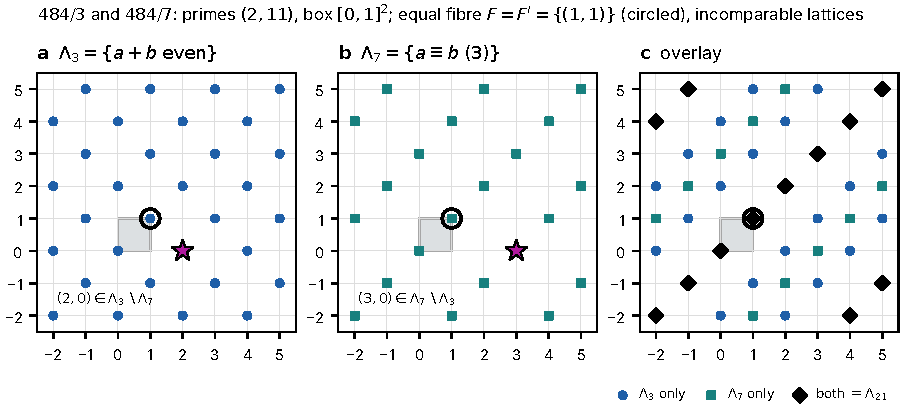
\includegraphics[width=0.98\textwidth]{fig02_equal_fibres}
\caption{Equal fibres, incomparable lattices (\cref{prop:fibre-vs-lattice}(b); \emph{exact computation}): $x=484/3$ and $x'=484/7$, primes $(2,11)$, box $[0,1]^2$, window $[-2,5]^2$ of the infinite lattices. (a)~$\Lambda_3=\{a+b\ \text{even}\}$; (b)~$\Lambda_7=\{a\equiv b\ (3)\}$; (c)~overlay, with $\Lambda_3\cap\Lambda_7=\Lambda_{21}$. The shaded unit square is the box and the point $(1,1)$ is the common fibre $F=F'$. The stars are the exact witnesses $(2,0)\in\Lambda_3\setminus\Lambda_7$ and $(3,0)\in\Lambda_7\setminus\Lambda_3$: the lattices are incomparable although the fibres coincide, so the spanning hypothesis in \cref{prop:fibre-vs-lattice}(c) cannot be dropped.}\label{fig:equalfibres}
\end{figure}
\begin{proof}
(a) is immediate. (c): $F\subseteq F'\subseteq\Lambda'$; take the span. (b): $484=2^2\cdot11^2$, so $d^2\mid484$ iff $d\mid22$; $22\equiv1$ modulo $3$ and $7$, while $2,11\not\equiv1$; thus $D=D'=\{22\}$, $F=F'=\{(1,1)\}$ for the box $[0,1]^2$. Modulo $3$: $2\equiv11\equiv-1$, so $\chi_3(a,b)=(-1)^{a+b}$. Modulo $7$: $2$ has order $3$ and $11\equiv2^2$, so $\chi_7(a,b)=2^{a+2b}$, trivial iff $a\equiv b\pmod 3$. Then $(2,0)\in\Lambda_3\setminus\Lambda_7$ and $(3,0)\in\Lambda_7\setminus\Lambda_3$. \qedhere
\end{proof}
The adapted statement (c) is the content of Lemma E2-4 (``no shrinking''): along a collective step with $D(x)\subseteq D(\Cmap(x))$ (Foundations Vol.~II, Thm.~1.3, F.T31~\cite{FoundII}; cited, not reproved) one has $F\subseteq F'$, so a spanning fibre forces $\Lambda\subseteq\Lambda'$. Also, every denominator along an orbit divides $G(x_0)$ (E2-3, resting on the same inherited facts), so the lattices along an orbit all contain $\Lambda_{G(x_0)}$ in fixed coordinates. The spanning hypothesis must accompany every use of (c) (ER-14).
\prov{CW-0458}{E2-3}{PROVED}{ADAPTED}

\subsection{Corpus statistics (finite-exact)}
\begin{proposition}[FINITE-EXACT; source scope]\label{prop:corpus}
In the exact corpus of $596$ admissible non-EQUAL transitions of the source ($582$ with $k=2$, $14$ with $k=3$) one finds ENLARGE $275$, SHRINK $262$, INCOMPARABLE $59$; in every row $F\subseteq F'$. No SHRINK or INCOMPARABLE row has a spanning source fibre ($321/321$). If $b\mid b'$ the class is SHRINK in all $199$ such rows; if $b'\mid b$ it is ENLARGE in all $154$.
\end{proposition}
\prov{CW-0472}{P2-D}{FINITE-EXACT}{FINITE}
These numbers are a computation in the stated corpus, reported from the release; the planar sampling windows of the first release were incomplete for boxes with $q_1<q_2$, and all $326$ geometry verdicts were recomputed with full-box certificates in the next release with $0$ verdicts changed (ER-18); they are not re-derived here and are not extrapolated. Their consequence for this manuscript is only qualitative: transitions with SHRINK or INCOMPARABLE lattices occur under $\Cmap$ (so ``the lattice never shrinks'' is not a law, ER-14), and transport theorems must either assume $\Lambda\subseteq\Lambda'$ or avoid lattice comparison.

\section{Abstract transport of cells}\label{sec:cells}

\subsection{Region Graver sets and the survival criterion}
\begin{lemma}\label{lem:regionG}
For every lattice $\Lambda\subseteq\Z^k$, $\Gr_q(\Lambda)=\{g\in\Gr(\Lambda):|g_i|\le q_i\ \forall i\}$.
\end{lemma}
\prov{CW-0466}{P2-L1}{PROVED}{FULL}
\begin{proof}
If $h\cm g$ and $|g_i|\le q_i$ then $|h_i|\le q_i$, so every conformal subvector of a vector of the box lies in the box; minimality within the box and within $\Lambda$ coincide for vectors of the box. \qedhere
\end{proof}
\begin{theorem}[generator survival without the target complex]\label{thm:P2T2}
Let $g\in\Gr_q(\Lambda)$. Then $g\in\Gr_q(\Lambda')$ iff $g\in\Lambda'$ and no $v\in\Lambda'\setminus\{0,g\}$ satisfies $v\cm g$. Only $\prod_i(|g_i|+1)-2$ candidate vectors $v$ have to be inspected, and only $\chi_{b'}$ is needed.
\end{theorem}
\prov{CW-0469}{P2-T2}{PROVED}{FULL}
\begin{proof}
Definition of conformal minimality and \cref{lem:regionG}; the candidates are the integer points of the conformal box of $g$. \qedhere
\end{proof}
\begin{theorem}[abstract-cell transport]\label{thm:cell-transport}
Let $\Lambda,\Lambda'$ be lattices, $Q$ a common box, and $c$ a cell of $\Kabs(\Lambda,Q)$. Then
\[
c\in\Kabs(\Lambda',Q)\iff V(c)\subseteq F(\Lambda',Q)\ \text{and}\ \mathrm{Gen}(c)\subseteq\Gr_q(\Lambda').
\]
Put $S=\Gr_q(\Lambda)\cap\Gr_q(\Lambda')$. Then (1) if $\Lambda\subseteq\Lambda'$ all $0$-cells persist, and a $j$-cell $c$ persists iff $\mathrm{Gen}(c)\subseteq S$; (2) no cell of dimension $>\rk\langle S\rangle$ persists; in particular $S=\emptyset$ implies that all cells of positive dimension are lost, and $\rk\langle S\rangle=1$ implies that all $2$-cells are lost; (3) if $\Gr_q(\Lambda)\subseteq\Gr_q(\Lambda')$ and $\Lambda\subseteq\Lambda'$ then $\Kabs(\Lambda,Q)\subseteq\Kabs(\Lambda',Q)$.
\end{theorem}
\prov{CW-0470}{P2-T3}{PROVED}{FULL}
\begin{proof}
($\Rightarrow$) If $c$ is a cell of $\Kabs(\Lambda',Q)$ its vertices are in $F(\Lambda',Q)$ and, by \cref{lem:intrinsic}, $\mathrm{Gen}(c)$ is the set of edge vectors at its smallest vertex (up to sign), which lie in $\Gr_q(\Lambda')$ as generators of a cell of $\Lambda'$. ($\Leftarrow$) Let $m$ be the smallest vertex of $c$. Then $\Pil(m;\mathrm{Gen}(c))$ has independent generators in $\Gr_q(\Lambda')$ and all corners in $V(c)\subseteq F(\Lambda',Q)$, so it is a cell of $\Lambda'$; it has vertex set $V(c)$, hence equals $c$. (1)--(3): for $\Lambda\subseteq\Lambda'$ the vertex condition is automatic; a cell with $j$ independent generators in $S$ needs $j\le\rk\langle S\rangle$; (3) is (1) read for all cells. \qedhere
\end{proof}
This is the general form of the survival rule (ER-15): the earlier statement that a cell survives iff its generators lie in $\Gr\cap\Gr'$ is correct only when its vertices already lie in $F'$, as they do for $\Lambda\subseteq\Lambda'$.

\subsection{Graver sets of \texorpdfstring{$\Z^k$}{Z\^{}k} and of the even-sum lattice}
\begin{proposition}\label{prop:E25}
For $k\ge2$: $\Gr(\Z^k)=\{\pm e_i\}$ and $\Gr(E_k)=\{\pm2e_i\}\cup\{\pm e_i\pm e_j:i<j\}$. The two sets are disjoint.
\end{proposition}
\prov{CW-0460}{E2-5}{PROVED}{FULL}
\begin{proof}
In $\Z^k$ each $e_i$ is minimal, and any nonzero vector dominates some $\pm e_i$. In $E_k$: $e_i\notin E_k$, so $2e_i$ and $e_i\pm e_j$ have no proper nonzero conformal lattice subvector (the only candidates are $\pm e_i,\pm e_j$), hence are minimal. Conversely let $0\ne\lambda\in E_k$. If $|\lambda_i|\ge2$ for some $i$ and $\lambda\ne\pm2e_i$, then $2\,\mathrm{sign}(\lambda_i)e_i\prec\lambda$ is a lattice vector, so $\lambda$ is not minimal. If all $|\lambda_i|\le1$, the support has even size $\ge2$; if it has $\ge4$ elements, then $\mathrm{sign}(\lambda_i)e_i+\mathrm{sign}(\lambda_j)e_j\prec\lambda$ for two support indices. \qedhere
\end{proof}
(The set $\Gr(E_k)$ is the root system $D_k$ together with $\pm2e_i$.)

\subsection{The three-stage orbit}\label{sec:threestage}
\begin{theorem}[three-stage orbit; all $k$, all admissible prime sets]\label{thm:E21}
Let $k\ge2$, $p_1=2<p_2<\dots<p_k$ primes with $p_i\equiv2\pmod 3$, $P=\prod p_i$, $x_0=P^4/3$. Then $L(x_0)=P^2$, $G(x_0)=3$, $x_1=\Cmap(x_0)=2P^4/3$, $x_2=\Cmap(x_1)=P^4$, and
\begin{center}\small
\begin{tabular}{@{}lccc@{}}\toprule
 & $x_0$ & $x_1$ & $x_2$\\\midrule
reduced denominator & $3$ & $3$ & $1$\\
box $q$ & $(2,\dots,2)$ & $(2,\dots,2)$ & $(2,\dots,2)$\\
$|F|$ & $(3^k-1)/2$ & $(3^k-1)/2$ & $3^k-1$\\
relation lattice & $E_k$ & $E_k$ & $\Z^k$\\
$D$ & $D_0$ & $=D_0$ & $\supsetneq D_0$\\\bottomrule
\end{tabular}
\end{center}
\end{theorem}
\prov{CW-0456}{E2-1}{PROVED}{FULL}
\begin{proof}
$d^2\mid P^4\iff d\mid P^2$, so $d=\prod p_i^{\alpha_i}$ with $\alpha\in\{0,1,2\}^k$. Since $p_i\equiv-1\pmod3$, $d\equiv(-1)^{\sum\alpha_i}$; thus $D(x_0)$ corresponds to the nonzero even-weight vectors, $(3^k+1)/2-1=(3^k-1)/2$ of them. The vectors $2e_i$ (that is, $d=p_i^2$) lie in $D(x_0)$ and every $d$ divides $P^2$, so $L=P^2$. Every $d-1$ is divisible by $3$, and $4=2^2\in D(x_0)$ has $d-1=3$, so $G=3$. Hence $\Cmap(x_0)=P^4/3+P^4/3=2P^4/3$. In $x_1$ the numerator $2P^4$ is prime to $3$ and $v_2(2P^4)=5$, $\lfloor5/2\rfloor=2$; the active primes, the box, and (since $d^2\mid2P^4\iff d\mid P^2$) the set $D$ are unchanged, so are $L,G$, and $\Cmap(x_1)=2P^4/3+P^4/3=P^4$. For $x_2=P^4$ the denominator is $1$, $D(x_2)$ is the set of all divisors $\ge2$ of $P^2$ ($3^k-1$ of them) and the lattice is $\Z^k$. \qedhere
\end{proof}
\begin{corollary}[all positive-dimensional cells are lost]\label{cor:threestage}
For the transition $x_1\to x_2$ of \cref{thm:E21} and every $k\ge2$: all vertices persist, no cell of positive dimension of $\Kabs(E_k,Q)$ is a cell of $\Kabs(\Z^k,Q)$, although $D(x_1)\subsetneq D(x_2)$. The transition $x_0\to x_1$ is the identity on $(\Lambda,Q)$.
\end{corollary}
\prov{CW-0461}{E2-6}{PROVED}{FULL}
\begin{proof}
$E_k\subseteq\Z^k$ gives $F\subseteq F'$. By \cref{prop:E25} $S=\Gr(E_k)\cap\Gr(\Z^k)=\emptyset$ (the boxes $[-2,2]^k$ contain all of both Graver sets), so \cref{thm:cell-transport}(2) applies. \qedhere
\end{proof}
The corollary generalises the specimen $P=110$, $k=3$, in which $13\to13\to26$ points; that specimen has the following exact counts, obtained here by independent exact code (\texttt{scripts/run\_exact\_checks.py}).
\begin{proposition}[specimen $k=3$, FINITE-EXACT]\label{prop:specimen}
For $\Lambda=E_3$ and $\Lambda'=\Z^3$ with $Q=[0,2]^3$: the f-vectors of $\Kabs$ are $(13,45,36,3)$ and $(26,51,33,7)$; the Betti numbers over $\Q$ are $(1,6,6,0)$ and $(1,0,0,0)$; of the source cells $0$ edges, $0$ squares, $0$ cubes persist, with $45,36,3$ lost and $51,33,7$ new.
\end{proposition}
\prov{CW-0464}{E2-10}{FINITE-EXACT}{FINITE}
\noindent These are counts for one specimen ($k=3$, box $[0,2]^3$), obtained by exhaustive enumeration, with $\partial\partial=0$ checked. The Betti numbers of the realised union $U$ ($(1,0,18,0)$ for the source and $(1,0,0,0)$ for the target) and the statement that $\Kabs(E_3,Q)$ is not embedded are reported by the release from an exact nerve computation and are cited, not re-derived here; the realised $b_2=18$ differs from the abstract $b_2=6$, which is why every topological statement must name its object.
\begin{figure}[tbp]\centering
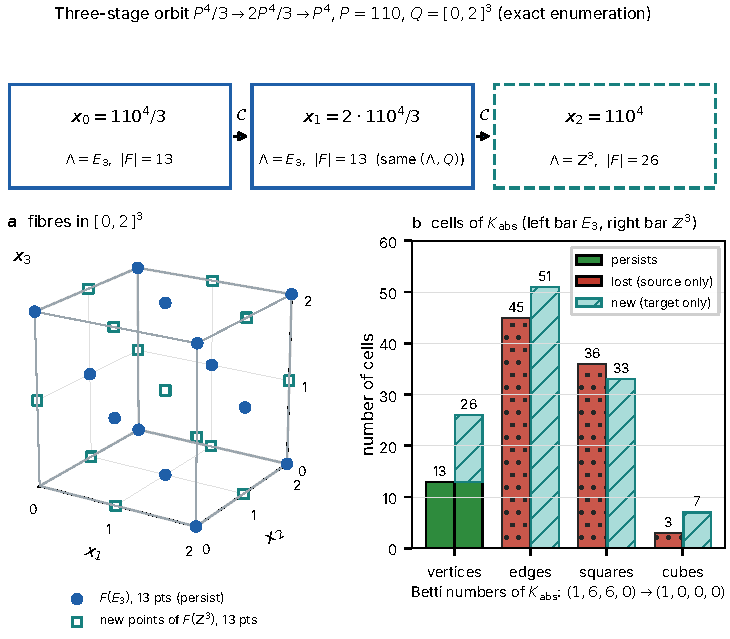
\includegraphics[width=0.78\textwidth]{fig03_three_stage}
\caption{The three-stage orbit $P^4/3\to2P^4/3\to P^4$ for $P=110$, $k=3$, $Q=[0,2]^3$ (\cref{thm:E21,cor:threestage,prop:specimen}; \emph{exact computation}). The first step is the identity on $(\Lambda,Q)=(E_3,Q)$; the second enlarges $E_3$ to $\Z^3$ ($13\to13\to26$ occurrences). (a)~Fibres: the $13$ points of $F(E_3,Q)$ persist, $13$ new points of $F(\Z^3,Q)$ appear. (b)~Cell counts of the abstract complexes $\Kabs(E_3,Q)$, f-vector $(13,45,36,3)$, and $\Kabs(\Z^3,Q)$, f-vector $(26,51,33,7)$: all $13$ vertices persist (green) and no positive-dimensional cell does (red: lost; hatched teal: new). The abstract Betti numbers change from $(1,6,6,0)$ to $(1,0,0,0)$. Only abstract complexes are counted; the realised unions are compared in \cref{sec:realised}.}\label{fig:threestage}
\end{figure}

\subsection{A planar family with exact edge counts}
\begin{theorem}\label{thm:P2TF1}
Let $x_h=21^{2h}/5$, $h\ge1$. (i) $D(x_h)=\{3^a7^b:a\equiv b\ (4),\ 0\le a,b\le h,\ (a,b)\ne0\}$, $L=21^h$, $G=20$, $\Cmap(x_h)=x_h'=21^{2h}/4$; the primes $(3,7)$ and the box $(h,h)$ are unchanged. (ii) $\Lambda=\{a\equiv b\ (4)\}\subsetneq\Lambda'=\{a\equiv b\ (2)\}$. (iii) $\Gr(\Lambda)=\pm\{(1,1),(4,0),(0,4),(1,-3),(3,-1),(2,-2)\}$, $\Gr(\Lambda')=\pm\{(1,1),(1,-1),(2,0),(0,2)\}$, and $\Gr_h(\Lambda)\cap\Gr_h(\Lambda')=\{\pm(1,1)\}$ for every $h\ge1$. (iv) All vertices persist; the persisting edges are exactly the edges $\{u,u+(1,1)\}$; no $2$-cell persists; their number is
\[
E_{\mathrm{kept}}(h)=\sum_{r=0}^3c_r(h)^2-1,\qquad c_r(h)=\#\{n\in[0,h-1]:n\equiv r\ (4)\}.
\]
\end{theorem}
\prov{CW-0471}{P2-TF1}{PROVED}{FULL}
\begin{proof}
(i) $d^2\mid21^{2h}$ iff $d\mid21^h$, $d=3^a7^b$. Modulo $5$: $7\equiv2\equiv3^3$ and $3$ has order $4$, so $3^a7^b\equiv3^{a+3b}\equiv3^{a-b}$, which is $1$ iff $a\equiv b\ (4)$. Then $(h,h)\in D$, so $L=21^h$. Every such $d$ has $a+b$ even; since $3\equiv7\equiv-1\pmod4$ we get $d\equiv1\pmod4$, with $5\mid d-1$: $20\mid G$. And $21\in D$ ($a=b=1$) has $21-1=20$, so $G=20$. Therefore $\Cmap(x_h)=21^{2h}(\tfrac15+\tfrac1{20})=21^{2h}/4$; the numerator is unchanged, so primes and box are unchanged. (ii) Modulo $4$: $3^a7^b\equiv(-1)^{a+b}$; modulo $5$ as in (i). (iii) Let $v=(a,b)\ne0$ in $\Lambda$. If $a,b\ge1$ then $(1,1)\cm v$; if $b=0$ then $4\mid a$ and $(4,0)\cm v$; likewise $a=0$. If $a>0>b$ put $c=-b>0$, so $a+c\equiv0\ (4)$; $a\ge4$ gives $(4,0)\cm v$ and $c\ge4$ gives $(0,-4)\cm v$, so minimal vectors have $a,c\le3$ and $a+c=4$: $(1,-3),(2,-2),(3,-1)$, each minimal because every nonzero proper conformal subvector has $a'+c'\in\{1,2,3\}$. For $\Lambda'$: this is $\Gr(E_2)$ by \cref{prop:E25}. The source vectors $(4,0),(0,4),(1,-3),(3,-1),(2,-2)$ dominate $(2,0),(0,2),(1,-1),(1,-1),(1,-1)$ respectively, all in $\Lambda'$, so they are not target Graver vectors; $(1,1)$ is common; the target vectors $(1,-1),(2,0),(0,2)$ are not in $\Lambda$. Region sets are the intersections with $[-h,h]^2$ (\cref{lem:regionG}); $(1,1)$ lies in the box for $h\ge1$. (iv) $\Lambda\subseteq\Lambda'$ gives $F\subseteq F'$. By \cref{thm:cell-transport} an edge persists iff its generator is in $S=\{\pm(1,1)\}$, and a $2$-cell needs two independent generators in $S$: impossible. The $(1,1)$-edges are $\{u,u+(1,1)\}$ with $u=(a,b)$, $a\equiv b\ (4)$, $0\le a,b\le h-1$, $u\ne0$; counting residue classes gives $\sum c_r^2-1$. \qedhere
\end{proof}
\begin{remark}
The release also gives closed quasi-polynomial formulas for the number of source and target edges and the limiting survival ratio $1/6$; the quasi-polynomials for the source and target edge counts are valid only for $h\ge4$ (ER-17), whereas $E_{\mathrm{kept}}(h)$ above holds for all $h\ge1$. Those counting formulas are not reproduced here. For $h=1,\dots,12$ the value $E_{\mathrm{kept}}$, the equality $S=\{\pm(1,1)\}$ and the non-persistence of $2$-cells were confirmed by direct exact enumeration (\texttt{scripts/run\_exact\_checks.py}); this confirms the proof and is not a substitute for it. \Cref{fig:planar} shows $h=8$.
\end{remark}
\begin{figure}[tbp]\centering
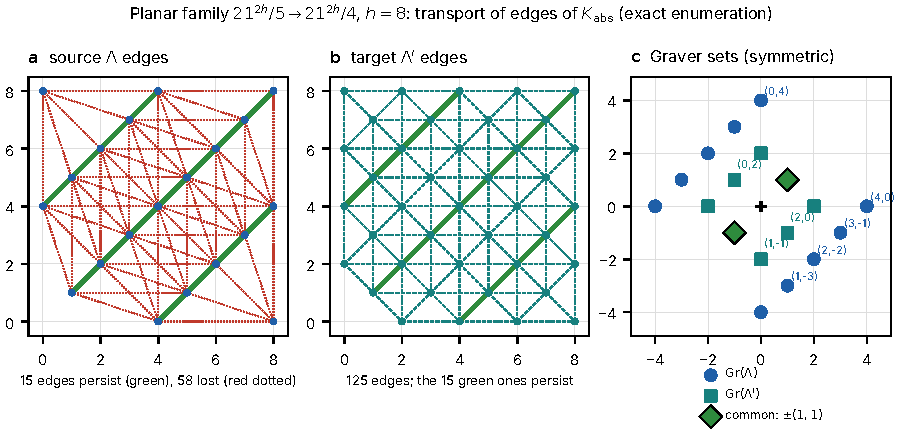
\includegraphics[width=0.98\textwidth]{fig04_planar_edges}
\caption{Planar family $21^{2h}/5\to21^{2h}/4$ for $h=8$ (\cref{thm:P2TF1}; \emph{exact computation} of $\Kabs$). (a)~The $73$ edges of $\Kabs(\Lambda,Q)$, $\Lambda=\{a\equiv b\ (4)\}$: the $15=E_{\mathrm{kept}}(8)$ edges with generator $\pm(1,1)$ persist (green, thick) and the other $58$ are lost (red, dotted). (b)~The $125$ edges of $\Kabs(\Lambda',Q)$, $\Lambda'=\{a\equiv b\ (2)\}$, with the persisting edges again green. (c)~The Graver sets $\Gr(\Lambda)$ and $\Gr(\Lambda')$ (each symmetric under $v\mapsto-v$) in the window $[-4,4]^2$; they share only $\pm(1,1)$, which is why only $(1,1)$-edges can persist (\cref{thm:cell-transport}). The panels show abstract complexes (edges only), not the realised unions.}\label{fig:planar}
\end{figure}

\section{Rectangular targets and the corner cube}\label{sec:corner}
The simplest target is rectangular: $\Lambda'=\bigoplus_io_i\Z$, which has Graver set $\{\pm o_ie_i\}$. This includes $\Lambda'=\Z^k$ (all $o_i=1$), the case $b'=1$. For rectangular targets the realised union has an explicit complement and the transport question becomes exact.

\subsection{Gap reduction}
\begin{lemma}[coverage-gap reduction]\label{lem:gap}
Let $F\subseteq F'$ and let $H=\conv F\subseteq H'=\conv F'$. Put $\mathcal G'=H'\setminus U'$. Then $U\setminus U'=U\cap\mathcal G'$. Hence $U\subseteq U'\iff U\cap\mathcal G'=\emptyset$, and $U'=H'$ implies $U\subseteq U'$.
\end{lemma}
\prov{CW-0476}{P3-T0}{PROVED}{FULL}
\begin{proof}
Every cell is the convex hull of its vertices, so $U\subseteq H\subseteq H'$. A point of $U$ outside $U'$ therefore lies in $H'\setminus U'$, and conversely. \qedhere
\end{proof}

\subsection{The corner-cube criterion}
Fix a rectangular target $\Lambda'=\bigoplus o_i\Z$, a source $\Lambda$ with $F(\Lambda,Q)\subseteq F(\Lambda',Q)$, and assume $\tilde Q_i=\lfloor q_i/o_i\rfloor\ge1$ for all $i$ (if some $\tilde Q_i=0$, the coordinate carries no point of $F'\supseteq F$ and the problem is the same problem in $k-1$ coordinates). Put $A_i=o_i\tilde Q_i$, $B=\prod[0,A_i]$ and let $O=\{z\in\R^k:z_i<o_i\ \forall i\}$ be the \emph{open corner cube}.
\begin{theorem}[corner-cube criterion]\label{thm:corner}
(a) $U'=B\setminus O=\{z\in B:\max_iz_i/o_i\ge1\}$.
(b) $U\subseteq U'\iff U\cap O=\emptyset\iff$ no cell of $\Kabs(\Lambda,Q)$ meets $O$.
(c) If $U\cap O\ne\emptyset$, the scaled lattice $\tilde\Lambda=\mathrm{diag}(o)^{-1}\Lambda$ contains a nonzero vector $v\ge0$ with $|v|_1\le k-1$.
(d) No cell of dimension $\le1$ meets $O$, in any dimension $k$.
(e) If $k=2$ then $U\subseteq U'$ (for every rectangular target, including $\Z^2$).
(f) If a $k$-cell meets $O$, then one of its $(k-1)$-faces (itself a cell) meets $O$. Hence for $k=3$ every obstruction is carried by a $2$-cell.
\end{theorem}
\prov{CW-0479}{P3-T3}{PROVED}{FULL}
\begin{proof}
(a) The Graver vectors of $\Lambda'$ in $[-q,q]$ are $\pm o_ie_i$, so the cells of $\Kabs(\Lambda',Q)$ are the faces $\prod I_i$ of the grid cubes $\prod[n_io_i,(n_i+1)o_i]$ ($0\le n_i<\tilde Q_i$), with $I_i$ either an endpoint or the interval, all of whose corners are nonzero. ($\supseteq$) Let $z\in B$ with $z_{i_0}\ge o_{i_0}$ for some $i_0$. Put $I_i=\{z_i\}$ if $z_i/o_i\in\Z$ and $I_i=[n_io_i,(n_i+1)o_i]$ with $n_i=\lfloor z_i/o_i\rfloor$ otherwise (then $z_i<A_i$, so $(n_i+1)o_i\le A_i$). Then $\Phi=\prod I_i$ is a grid face containing $z$ whose every vertex has $i_0$-th coordinate $\ge o_{i_0}>0$ (if $I_{i_0}$ is an interval then $n_{i_0}\ge1$; otherwise $I_{i_0}=\{z_{i_0}\}$); so $0$ is not a vertex of $\Phi$, $\Phi$ is a cell, and $z\in U'$. ($\subseteq$) A cell is a grid face $\prod I_i$ that does not have $0$ as a vertex; $0$ is a vertex iff every $I_i$ has lower endpoint $0$, so some $I_i\subseteq[o_i,\infty)$ and every point of the cell has $z_i\ge o_i$.

(b) $U\subseteq H\subseteq\conv F'\subseteq B$, so $z\in U\setminus U'$ iff $z\in U\cap O$ by (a).

(c) Let $z\in U\cap O$ lie in a cell with vertices $v^{(j)}\in F\subseteq\Lambda$ and $z=\sum\lambda_jv^{(j)}$ (convex). In scaled coordinates $\tilde v^{(j)}\in\N^k\setminus\{0\}$ and $\sum_i\tilde z_i<k$ because each $\tilde z_i<1$, while $\sum_i\tilde z_i=\sum_j\lambda_j|\tilde v^{(j)}|_1$. So some vertex has $|\tilde v|_1<k$.

(d) A $0$-cell is a nonzero point of $\N^k$ in scaled coordinates, hence has a coordinate $\ge1$ and is not in $O$. Let $[P,R]$ be an edge, $P,R\in F$, $g=R-P\in\Gr(\Lambda)$ (either orientation), and suppose $z=(1-t)P+tR\in O$. In scaled coordinates $\tilde z_i<1$ forces $\tilde P_i=0$ or $\tilde R_i=0$ for each $i$ (if both were $\ge1$, then $\tilde z_i\ge1$): the supports are disjoint. Then $\tilde g=\tilde R-\tilde P$ agrees with $\tilde R$ on $\supp\tilde R$ and is $\le0$ where $\tilde P\ne0$, so $R\cm g$, $R\in\Lambda\setminus\{0\}$, and $R\ne g$ because $P\ne0$. Thus $g$ is not conformally minimal, a contradiction.

(e),(f) Let $C$ be a $k$-cell with $C\cap O\ne\emptyset$ and suppose $\partial C\cap O=\emptyset$. The cube $O$ is connected and $O=(O\cap\mathrm{int}\,C)\sqcup(O\setminus C)$ with both parts open, the first nonempty; so $O\subseteq\mathrm{int}\,C$ and $0\in\overline O\subseteq C$. All vertices of $C$ lie in the closed orthant, hence so does $C$; $0$ is an extreme point of the orthant, so $0$ is an extreme point of $C$, i.e.\ a vertex, but vertices lie in $F\not\ni0$. This contradiction shows $\partial C\cap O\ne\emptyset$; $\partial C$ is the union of the $(k-1)$-faces, which are cells. For $k=2$ these faces are edges, which miss $O$ by (d); cells of dimension $\le1$ miss $O$ by (d); so $U\cap O=\emptyset$ and (b) gives $U\subseteq U'$. \qedhere
\end{proof}
\begin{remark}[why dimension two is special]\label{rem:dim}
By (c) a failure needs a nonzero vertex of $\ell_1$-size at most $k-1$ in scaled coordinates. For $k=2$ this means a scaled vertex $e_i$, a configuration already excluded by (d)--(e); for $k=3$ the size $2$ is reached by vectors such as $(1,1,0)$, which exist in the even-sum lattice, and by (f) the cells that obstruct are squares. This is the first place where dimension enters; the planar hard-cell mechanism of \cref{sec:planar} is its non-rectangular analogue.
\end{remark}
\begin{figure}[tbp]\centering
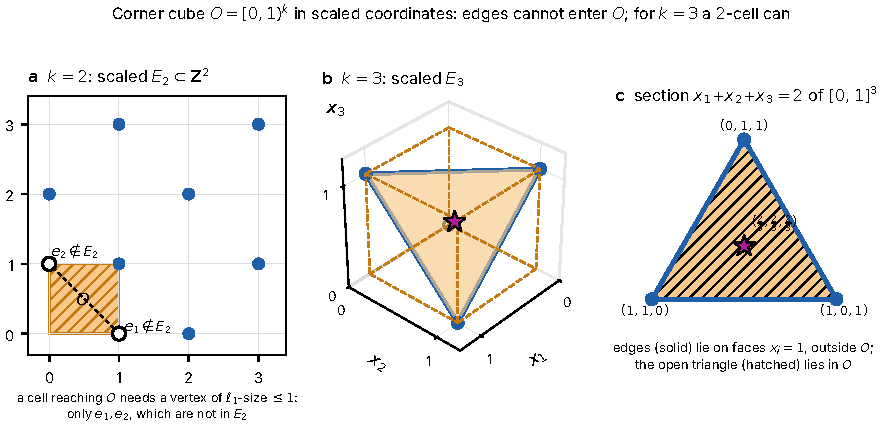
\includegraphics[width=0.98\textwidth]{fig05_dim2_vs_dim3}
\caption{Why dimensions two and three differ (\cref{thm:corner}(c)--(f), \cref{rem:dim}; scaled coordinates; \emph{theorem-level construction with exact coordinates}). (a)~$k=2$, scaled source $E_2\subset\Z^2$: a cell reaching the corner square $O=[0,1)^2$ would need a nonzero vertex of $\ell_1$-size $\le1$, i.e.\ $e_1$ or $e_2$, neither of which lies in $E_2$. (b)~$k=3$, scaled source $E_3\subset\Z^3$: the points $(1,1,0),(1,0,1),(0,1,1)$ of $\ell_1$-size $2$ \emph{do} lie in $E_3$; their triangle has its edges on faces $x_i=1$ of the unit cube, hence outside $O$, but its relative interior lies in $O$. The star is the centroid $(\frac23,\frac23,\frac23)$. (c)~The same triangle in the section $x_1+x_2+x_3=2$. The triangle is not a cell by itself; in \cref{fig:corner} it is part of the $2$-cell of $\Kabs(E_3,Q)$ that realises the obstruction.}\label{fig:dim}
\end{figure}

\subsection{The even-sum source}
\begin{theorem}[parametric obstruction for the even-sum family]\label{thm:evensum}
Let $k=3$, let $\Lambda'$ be rectangular and let the scaled source lattice be $E_3$ (index $2$), box $\tilde Q\ge(1,1,1)$. Then $U\not\subseteq U'$ iff $\max_i\tilde Q_i\ge2$. The smallest failing scaled box is $(1,1,2)$ up to permutation.
\end{theorem}
\prov{CW-0480}{P3-T3(h)}{PROVED}{FULL}
\begin{proof}
Both scalings by $\mathrm{diag}(o)^{-1}$ preserve the conformal order, Graver sets, cells, and the relation $U\subseteq U'$, so we work in scaled coordinates: $\Lambda=E_3$, $\Lambda'=\Z^3$, box $\tilde Q$. ($\Leftarrow$) Say $\tilde Q_3\ge2$. By \cref{prop:E25}, $g=(0,1,-1)$ and $h=(1,0,-1)$ are Graver vectors of $E_3$. The points $(0,0,2),(0,1,1),(1,0,1),(1,1,0)$ have even sum, are nonzero and lie in the box, so $\Pil((0,0,2);g,h)$ is a $2$-cell. Its point $(0,0,2)+\tfrac23g+\tfrac23h=(\tfrac23,\tfrac23,\tfrac23)$ lies in $O$, so $U\not\subseteq U'$ by \cref{thm:corner}(b). ($\Rightarrow$) If all $\tilde Q_i=1$, then $F=\{(1,1,0),(1,0,1),(0,1,1)\}$ ($(1,1,1)$ has odd sum): three points, so there is no $2$-cell; $U$ consists of points and edges, which miss $O$ by \cref{thm:corner}(d). \qedhere
\end{proof}
The cell and the point are drawn in \cref{fig:corner}. The first specimen of this phenomenon is the transition $13\to26$ of \cref{sec:threestage}, whose source cell $\Pil((0,0,2);(0,1,-1),(1,0,-1))$ is exactly this one.
\begin{figure}[tbp]\centering
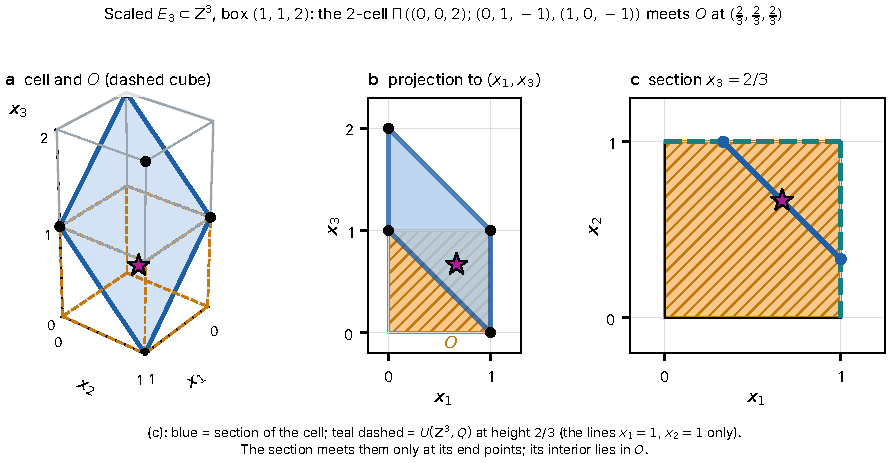
\includegraphics[width=0.98\textwidth]{fig06_corner_witness}
\caption{The exact corner-cube witness (\cref{thm:evensum}; scaled $\Lambda=E_3\subset\Lambda'=\Z^3$, box $(1,1,2)$; \emph{exact computation}). (a)~The $2$-cell $\Pil((0,0,2);(0,1,-1),(1,0,-1))$ of $\Kabs(E_3,Q)$ (a realised parallelogram), the five points of the fibre $F(E_3,Q)$ and the corner cube $O=[0,1)^3$ (dashed); the star is the witness $(\frac23,\frac23,\frac23)\in O$. (b)~Orthogonal projection to $(x_1,x_3)$, complementing the perspective view. (c)~The section $x_3=\frac23$: the section of the cell (blue segment from $(1,\frac13)$ to $(\frac13,1)$) has its interior in the open square $O$, while the target union $U(\Z^3,Q)$ at this height consists only of the lines $x_1=1$, $x_2=1$ (teal, dashed), met by the segment only at its end points. Hence the witness is not in $U(\Z^3,Q)$. All three panels show realised objects; none shows $\Kemb$.}\label{fig:corner}
\end{figure}

\subsection{The target union for \texorpdfstring{$b'=1$}{b\textquotesingle=1}}
\begin{corollary}[$U(\Z^k,Q)$]\label{cor:E27}
For $\Lambda'=\Z^k$ and $q\ge(1,\dots,1)$: $U(\Z^k,Q)=\{z\in Q:\max_iz_i\ge1\}$, a star-shaped (hence contractible) set. A convex polytope $\Pi\subseteq Q$ lies in it iff $\Pi\cap[0,1)^k=\emptyset$.
\end{corollary}
\prov{CW-0462}{E2-7}{PROVED}{ADAPTED}
\begin{proof}
\Cref{thm:corner}(a) with all $o_i=1$; star-shapedness about $q$: if $\max z_i\ge1$ then $\max(tz+(1-t)q)_i\ge1$ for $t\in[0,1]$ since $q_i\ge1$. \qedhere
\end{proof}
\begin{remark}[predictor]
For rectangular targets the criterion (b) can be evaluated cell by cell with one linear program per maximal source cell, never building the target complex. The release implements this; correctness is the content of (b). The procedure is an algorithm, not needed for the argument, and is not part of the theorem corpus of this manuscript (\texttt{CW-0481} is excluded for that reason).
\end{remark}
\prov{CW-0481}{P3-T4}{PROVED}{EXCLUDED}

\section{Realised transport: what abstract loss does and does not mean}\label{sec:realised}
\Cref{cor:threestage} says that the abstract complex of the three-stage orbit loses every positive-dimensional cell. This section shows that the realised union behaves differently: edges are always retained, some squares are not.

\subsection{Lost edges are geometrically retained}
\begin{theorem}\label{thm:E28}
Let $\Lambda\subseteq\Z^k$ be any lattice and $Q$ a box with all $q_i\ge1$. Every cell of dimension $\le1$ of $\Kabs(\Lambda,Q)$ lies in $U(\Z^k,Q)$. In particular, for the even-sum lattice $E_k$ every edge segment $[u,u+g]$, $g\in\Gr(E_k)$, of $\Kabs(E_k,Q)$ lies in $U(\Z^k,Q)$, although (\cref{cor:threestage}) none of these edges is an edge of $\Kabs(\Z^k,Q)$.
\end{theorem}
\prov{CW-0463}{E2-8}{PROVED}{FULL}
\begin{proof}
$\Z^k$ is a rectangular target with all $o_i=1$ and $F(\Lambda,Q)\subseteq F(\Z^k,Q)$. By \cref{thm:corner}(d) no cell of dimension $\le1$ meets $O=[0,1)^k$, and by \cref{thm:corner}(a)--(b) a subset of $B=Q$ that misses $O$ lies in $U(\Z^k,Q)$. \qedhere
\end{proof}
The release states and proves this for $E_k$ by a direct coordinate argument; the form above is the corner-cube form of the same fact. For the specimen $k=3$, all $45$ lost edges were also tested at five interior points each by independent code (a check of the theorem, not an additional proof).
\begin{figure}[tbp]\centering
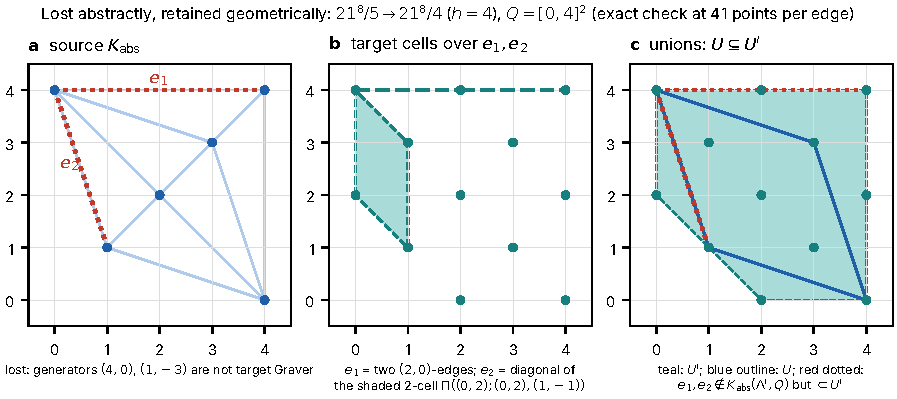
\includegraphics[width=0.98\textwidth]{fig07_lost_edges_retained}
\caption{Abstract loss versus realised containment (\cref{thm:E28} and \cref{thm:laws}(L3); planar specimen $21^{8}/5\to21^{8}/4$, $h=4$, $Q=[0,4]^2$; \emph{exact computation}, each edge checked exactly at $41$ points). (a)~Two edges $e_1$ (from $(0,4)$ to $(4,4)$, generator $(4,0)$) and $e_2$ (from $(0,4)$ to $(1,1)$, generator $(1,-3)$) of $\Kabs(\Lambda,Q)$, $\Lambda=\{a\equiv b\ (4)\}$; neither generator is Graver for $\Lambda'=\{a\equiv b\ (2)\}$, so both edges are lost in $\Kabs(\Lambda',Q)$. (b)~In the target complex $e_1$ is the union of two $(2,0)$-edges and $e_2$ is a diagonal of the shaded $2$-cell $\Pil((0,2);(0,2),(1,-1))$. (c)~The unions: $U(\Lambda',Q)$ (teal) contains $U(\Lambda,Q)$ (blue outline), and the lost edges (red, dotted) lie inside it. Distinct objects: lost in $\Kabs(\Lambda',Q)$, contained in $U(\Lambda',Q)$.}\label{fig:lost}
\end{figure}

\subsection{Cells that leave the union}
\begin{proposition}\label{prop:E29}\sloppy
Let $k=3$, $Q=[0,2]^3$. The parallelogram $c_*=\Pil((0,0,2);(0,1,-1),(1,0,-1))$ is a $2$-cell of $\Kabs(E_3,Q)$ (its corners $(0,0,2),(0,1,1),(1,0,1),(1,1,0)$ lie in $F(E_3,Q)$ and its generators are Graver). It contains $(\tfrac23,\tfrac23,\tfrac23)=(0,0,2)+\tfrac23(0,1,-1)+\tfrac23(1,0,-1)\in[0,1)^3$. Hence $U(E_3,Q)\not\subseteq U(\Z^3,Q)$ although $F(E_3,Q)\subseteq F(\Z^3,Q)$. Conversely $(1,0,0)\in U(\Z^3,Q)\setminus U(E_3,Q)$.
\end{proposition}
\prov{CW-0464}{E2-10}{FINITE-EXACT}{FINITE}
\begin{proof}
The first part is \cref{thm:evensum} for $\tilde Q=(2,2,2)$ and \cref{cor:E27}. For the converse, every nonzero point of $E_3$ has coordinate sum $\ge2$, hence so has every point of $U(E_3,Q)\subseteq\conv F(E_3,Q)$, while $(1,0,0)$ is a point of $F(\Z^3,Q)$. \qedhere
\end{proof}
(The proposition is carried by the source record E2-9, whose row is the same \texttt{CW-0464} area; the classification of \emph{which} source cells leave $U'$ --- exactly six, three squares and three cubes, all containing the three points $(0,1,1),(1,0,1),(1,1,0)$ --- is a finite exact computation of the release and is cited, not re-derived.)

\subsection{Finite findings on topology and specimens}
\begin{proposition}[FINITE-EXACT; scope: the $k=3$ specimen and two planar specimens]\label{prop:topology}
(a) For the specimen of \cref{prop:specimen} the Betti numbers of the abstract complexes are $(1,6,6,0)\to(1,0,0,0)$ while the fibre grows; the realised union of the source has Betti numbers $(1,0,18,0)$ (nerve computation of the release; cited). (b) For the planar specimen $21^8/5\to21^8/4$ ($h=4$) all $8$ abstractly lost edges and the lost square lie in $U'$, with $U\subsetneq U'$, realised Betti $(1,2,0)\to(1,0,0)$ while the abstract Betti numbers are $(1,5,0)\to(1,2,6)$; neither complex is embedded. (c) For the planar specimen $55^{12}/27\to55^{12}/18$ all $5$ source edges persist, $U$ is embedded with Betti $(1,0,0)$, but $U'$ is non-embedded with realised Betti $(1,2,0)$ (abstract $(1,8,0)$): enlargement can create holes.
\end{proposition}
\prov{CW-0474}{P2-G}{FINITE-EXACT}{FINITE}
Statement (a) first half was recomputed here; the other items are reported by the release and are not re-derived. The planar hole creation and destruction in (b),(c) are explained by frozen planar theory (the source lattices sit at the exceptional hollow box $(d,d)$ or below the stabilisation threshold; ER-19), so they are an observation about transport, not new single-fibre topology.

\subsection{Verdict on the plausible laws}
\begin{theorem}[laws refuted by exact witnesses]\label{thm:laws}
None of the following is true in general. (L1) $D(x)\subseteq D(x')$ implies persistence of Graver edges. (L2) $F\subseteq F'$ implies $U\subseteq U'$. (L3) Abstract loss of a cell implies that the cell leaves the target union. (L4) Topology of the abstract complex or of the union is monotone under inclusion of occurrence sets. (L5) A change of denominator changes the relation lattice.
\end{theorem}
\prov{CW-0465}{E2-11}{COUNTEREXAMPLE}{EXAMPLE}
\begin{proof}
(L1): \cref{cor:threestage}. (L2): \cref{prop:E29}. (L3): \cref{thm:E28}. (L4): \cref{prop:specimen} and \cref{prop:topology}: $b_1(\Kabs)$ falls from $6$ to $0$ and $b_2(U)$ from $18$ to $0$ while $F$ grows from $13$ to $26$ points (finite-exact specimen). (L5): for the primes $5,17,29$ the lattices for $b=3$ and $b=12$ coincide (\cref{cor:denominators}); the release's family of $405$ transitions of the three-stage type records $276$ EQUAL steps with denominator changes of this kind (finite-exact, cited). \qedhere
\end{proof}
\prov{CW-0475}{E2-P2-V}{PROVED}{EXAMPLE}
The release records six preregistered propositions P2-F1--P2-F6, each refuted by an exact witness; among them P2-F4 (abstract edge loss with full geometric containment, $199$ corpus rows) is the planar form of (L3) and P2-F5 (the planar pattern extends to $k=3$) is refuted by the witness of \cref{prop:E29}. The other verdicts are cited from the release and are not used below.

\section{Planar monotonicity}\label{sec:planar}
This section proves that in the plane the realised union is monotone under every inclusion of relation lattices and every box. The proof has three parts: a decomposition of cells into smaller cells of the target (\cref{sec:tools}), an exact criterion for when a cell can leave the target (\cref{sec:zero}), and the geometry of the cells that satisfy that criterion (\cref{sec:lg,sec:p5p1}). \Cref{sec:g12} places the result relative to the inherited planar stabilisation theorem.

\subsection{Two tools: conformal decomposition and zonotopal tiling}\label{sec:tools}
\begin{lemma}[conformal decomposition]\label{lem:L1}
Every $v$ in a lattice $M$ is a finite sum of Graver vectors of $M$, each conformally $\cm v$.
\end{lemma}
\prov{CW-0499}{E2P4v5-L1}{PROVED}{FULL}
\begin{proof}
Induction on $|v|_1$. For $v=0$ the sum is empty. Otherwise the set of nonzero lattice vectors $\cm v$ is finite and nonempty; a member $g$ of minimal $\ell_1$-norm is Graver (a nonzero $w'\cm g$ would also be $\cm v$ and shorter). Now $v-g\cm v$ is shorter; apply induction and transitivity of $\cm$. \qedhere
\end{proof}
\begin{lemma}[explicit tiling]\label{lem:T0}
Let $v_1,\dots,v_n$ be nonzero integer vectors spanning a $d$-dimensional subspace, written in lattice coordinates of the span, and $Z(V)=\sum[0,1]v_i$. Then $Z(V)$ is covered by finitely many tiles $T_S$, with pairwise disjoint interiors, each a translate of a parallelotope $Z(V_S)=\sum_{i\in S}[0,1]v_i$ with $V_S$ linearly independent, and every vertex of every tile is a subset sum $\sum_{i\in A}v_i$.
\end{lemma}
\prov{CW-0500}{E2P4v5-T0}{PROVED}{ADAPTED}
\begin{proof}
If $n=d$, $Z(V)$ is one parallelotope. Otherwise choose integer heights $w_i$ so generic that for every $d$-subset $S$ with $\det V_S\ne0$ and every $i\notin S$ the lifted vector $\tilde v_i=(v_i,w_i)\in\R^{d+1}$ is not in $\mathrm{span}(\tilde v_s:s\in S)$ (finitely many hyperplanes in $w$ are avoided: the coefficient of $w_i$ is $1$). For such $S$ let $\nu_S$ be a normal of $\mathrm{span}(\tilde v_S)$, signed with negative last coordinate (nonzero: it is $\pm\det V_S$), $A_S=\{i\notin S:\nu_S\cdot\tilde v_i>0\}$ and $T_S=\sum_{i\in A_S}v_i+Z(V_S)$. The face of the lifted zonotope $\tilde Z=\sum[0,1]\tilde v_i$ on which a functional $\nu$ is maximal is $\sum_{\nu\cdot\tilde v_i>0}\tilde v_i+\sum_{\nu\cdot\tilde v_i=0}[0,1]\tilde v_i$; by genericity the facets of $\tilde Z$ are the sets $\sum_{i\in A_S}\tilde v_i+Z(\tilde v_S)$, and such a facet is \emph{lower} iff $\nu_S$ has negative last coordinate. The lower facets project onto $T_S$ injectively, and \emph{by the lifting lemma (\cref{lem:lift})} they cover the shadow $Z(V)$ with disjoint interiors; (c) is the definition of $T_S$. \qedhere
\end{proof}
\noindent\textbf{The lifting fact.} The covering property used above is the standard statement that the lower facets of a lifted polytope project onto its shadow with disjoint interiors (the regular subdivision induced by a lifting, \cite{Ziegler1995,DLRS2010}; it is the construction behind the Bohne--Dress correspondence for zonotopal tilings \cite{Bohne1992,RGZ1994,HRS2000,BLSWZ1999}). It is proved in \cref{app:lifting} (\cref{lem:lift}), so \cref{lem:T0} is PROVED in full; the qualification of the first version is withdrawn. The release also checks the lemma numerically (volume sum $=\sum_S|\det V_S|$ and point location for random configurations), which is evidence for the implementation, not part of the proof.

\subsection{The zero-vertex criterion}\label{sec:zero}
Let $\Lambda\subseteq\Lambda'\subseteq\Z^k$ be lattices and $Q$ a box.
\begin{proposition}[zero-vertex criterion]\label{prop:Z}
Let $c=\Pil(u;g_1,\dots,g_j)$ be a cell of $\Kabs(\Lambda,Q)$, and call \emph{zero-vertex decomposition} a choice of $s_i\in\Lambda'$ with $s_i\cm g_i$ (possibly $0$ or $g_i$) and $u+\sum s_i=0$.
\begin{enumerate}[label=(Z.\arabic*)]
\item If $c$ has no zero-vertex decomposition then $c\subseteq U(\Lambda',Q)$.
\item $c$ has a zero-vertex decomposition iff $m(c):=u+\sum_ig_i^-=0$ and $g_i^-\in\Lambda'$ for all $i$ (then $s_i=g_i^-$).
\item Every cell has $2^j$ representations (base corner and generator signs), and Z.1 applies to each. Hence $c\subseteq U(\Lambda',Q)$ unless $m(c)=0$ and $g_i^-\in\Lambda'$ for all $i$ (equivalently $g_i^+\in\Lambda'$, since $g_i\in\Lambda\subseteq\Lambda'$). Cells with this property are \emph{hard}.
\item There are no hard cells of dimension $\le1$ (edges never obstruct).
\end{enumerate}
\end{proposition}
\prov{CW-0501}{E2P4v5-Z}{PROVED}{FULL}
\prov{CW-0490}{P4-Z1}{PROVED}{FULL}
\prov{CW-0496}{P4-Z2}{PROVED}{FULL}
\prov{CW-0491}{P4-Z1.a}{PROVED}{FULL}
\begin{proof}
(Z.1) By \cref{lem:L1} write each $g_i=\sum_th_{i,t}$ with $h_{i,t}\in\Gr(\Lambda')$ and $h_{i,t}\cm g_i$. Then $Z'=u+\sum_{i,t}[0,1]h_{i,t}$ contains $c$ (for $\lambda_i\in[0,1]$, $\lambda_ig_i=\sum_t\lambda_ih_{i,t}$). Tile $Z'$ by \cref{lem:T0}. A vertex of a tile is $u+\sum_{(i,t)\in A}h_{i,t}=u+\sum_is_i$, where $s_i$ is a partial sum of the pieces of $g_i$; all pieces have the sign pattern of $g_i$, so $s_i\in\Lambda'$ and $s_i\cm g_i$. For each coordinate $\ell$ the vertex coordinate lies between $u_\ell+\sum_i\min(g_{i,\ell},0)$ and $u_\ell+\sum_i\max(g_{i,\ell},0)$, which are coordinates of two corners of $c$, hence in $[0,q_\ell]$: the vertex is in $Q$. It is nonzero by hypothesis. So every tile (generators $h_{i,t}$ Graver in $\Lambda'$ and in the box, independent, all vertices in $F(\Lambda',Q)$) is a cell of $\Lambda'$, and $c\subseteq Z'\subseteq U(\Lambda',Q)$.

(Z.2) ($\Rightarrow$) Coordinatewise $s_{i,\ell}\ge\min(g_{i,\ell},0)$, so $0=u_\ell+\sum_is_{i,\ell}\ge m_\ell$; but $m_\ell$ is a coordinate of the corner $u+\sum_{g_{i,\ell}<0}g_i$ of $c$, hence $\ge0$. So equality holds throughout: $m=0$ and $s_{i,\ell}=\min(g_{i,\ell},0)$, that is $s_i=g_i^-\in\Lambda'$. ($\Leftarrow$) Take $s_i=g_i^-\cm g_i$.

(Z.3) $m(c)$ is the coordinatewise minimum of the corners, independent of the representation; the representation with generators $\epsilon_ig_i$ has outgoing negative parts $(\epsilon_ig_i)^-\in\{g_i^-,-g_i^+\}$. All $2^j$ representations have a zero-vertex decomposition iff $m(c)=0$ and both $g_i^-$ and $g_i^+$ lie in $\Lambda'$ for every $i$.

(Z.4) If a cell $\Pil(u;g)$ were hard then $u+g^-=0$, so $-u=g^-$, a nonzero element of $\Lambda$ ($u\in F\subseteq\Lambda$) with $g^-\cm g$; and $g^-\ne g$, else $u+g=0\notin F$. This contradicts $g\in\Gr(\Lambda)$. Points are covered trivially. \qedhere
\end{proof}
The release gives (Z.1) and (Z.2) first as P4-Z1, P4-Z2 and then re-proves them with a complete argument as Z; the three records are merged here with one proof.

\subsection{Adjacent corners overlap in support}\label{sec:lg}
\begin{lemma}\label{lem:LG}
If $P,P'$ are corners of a cell of $U(\Lambda,Q)$ that differ by one generator $w=P'-P$, then $\supp P\cap\supp P'\ne\emptyset$.
\end{lemma}
\prov{CW-0502}{E2P4v5-LG}{PROVED}{FULL}
\begin{proof}
$P,P'$ are nonzero and $\ge0$. If the supports were disjoint then $P'\cm w$ and $-P\cm w$ (on $\supp P'$, $w_\ell=P'_\ell\ge0=P_\ell$; on $\supp P$, $w_\ell=-P_\ell\le0=P'_\ell$; zero elsewhere), both lie in $\Lambda$ and are nonzero, $P'\ne w$ (else $P=0$) and $-P\ne w$ (else $P'=0$): $w$ would not be Graver. \qedhere
\end{proof}

\subsection{The planar theorem}\label{sec:p5p1}
\begin{theorem}[planar monotonicity]\label{thm:planar}
Let $\Lambda\subseteq\Lambda'\subseteq\Z^2$ be lattices of rank $2$ and $Q=[0,a]\times[0,b]$ any box. Then $U(\Lambda,Q)\subseteq U(\Lambda',Q)$.
\end{theorem}
\prov{CW-0504}{P5-P1}{PROVED}{FULL}
\prov{CW-0497}{P4-P1}{PROVED}{FULL}
\begin{proof}
Points are trivial and edges are covered by \cref{prop:Z}(Z.4) and (Z.3). Let $c$ be a $2$-cell. If it is not hard, \cref{prop:Z}(Z.3) applies. Let it be hard. Let $k',l'\ge1$ be minimal with $k'e_1,l'e_2\in\Lambda'$ (they exist: finite index), so $\{t:te_1\in\Lambda'\}=k'\Z$. Then $k'e_1$ and $l'e_2$ are Graver in $\Lambda'$: a nonzero conformal subvector of $k'e_1$ in $\Lambda'$ is $(t,0)$ with $0<t\le k'$, so $t=k'$.
\begin{enumerate}[label=(\arabic*),leftmargin=*]
\item $m(c)=0$ gives a corner $A$ with $x=0$ and a corner $B$ with $y=0$; both are nonzero, so $A=(0,y_0)$, $B=(x_0,0)$ with $x_0,y_0>0$.
\item $\supp A=\{2\}$ and $\supp B=\{1\}$ are disjoint, so by \cref{lem:LG} $A,B$ are not adjacent: they are opposite corners. Let $D,E$ be the other two.
\item Write the edge vectors at $A$ as $g',h'$ with $B=A+g'+h'$, $D=A+g'$, $E=A+h'$. Since $D,E\in Q$: $g'_1,h'_1\ge0$ and $y_0+g'_2,y_0+h'_2\ge0$. As $g'_2+h'_2=-y_0$, both $g'_2,h'_2\le0$. Write $g'=(g_1,-g_2)$, $h'=(h_1,-h_2)$ with $g_1,g_2,h_1,h_2\ge0$, $g_1+h_1=x_0$, $g_2+h_2=y_0$; then $D=(g_1,h_2)$, $E=(h_1,g_2)$.
\item All four numbers are positive: $D$ is adjacent to both $A$ and $B$ and nonzero, so by \cref{lem:LG} $\supp D$ meets $\{2\}$ and $\{1\}$: $h_2>0$ and $g_1>0$. Likewise for $E$: $h_1>0$, $g_2>0$.
\item Hardness: $g'^{+}=(g_1,0)$, $g'^-=(0,-g_2)$, $h'^+=(h_1,0)$, $h'^-=(0,-h_2)$ lie in $\Lambda'$ (up to the sign convention of \cref{prop:Z}(Z.3)). Hence $k'\mid g_1,h_1$ and $l'\mid g_2,h_2$, so $g_1,h_1\ge k'$ and $g_2,h_2\ge l'$; $x_0=g_1+h_1\in k'\Z$, $x_0\ge2k'$, $y_0\in l'\Z$, $y_0\ge2l'$.
\item The four corners satisfy $x/k'+y/l'\ge2$ ($A$: $y_0/l'\ge2$; $B$: $x_0/k'\ge2$; $D$: $g_1/k'+h_2/l'\ge2$; $E$ likewise). By convexity every $p\in c$ has $p_1/k'+p_2/l'\ge2$, so \textbf{$p_1\ge k'$ or $p_2\ge l'$}.
\item The rectangles $R_{ij}=[ik',(i+1)k']\times[jl',(j+1)l']$, $0\le i<x_0/k'$, $0\le j<y_0/l'$, tile $[0,x_0]\times[0,y_0]\subseteq Q$ (the box contains the bounding box of the corners). Their corners lie in $k'\Z\times l'\Z\subseteq\Lambda'$, in $Q$, and are nonzero except the corner $0$ of $R_{00}$. So each $R_{ij}$, $(i,j)\ne(0,0)$, is the cell $\Pil(\text{corner};k'e_1,l'e_2)$ of $U(\Lambda',Q)$. A point $p\in c$ with $p_1\ge k'$ lies in some $R_{ij}$ with $i\ge1$ (because $x_0/k'\ge2$), and one with $p_2\ge l'$ lies in some $R_{ij}$ with $j\ge1$. Hence $c\subseteq U(\Lambda',Q)$. \qedhere
\end{enumerate}
\end{proof}
\begin{figure}[tbp]\centering
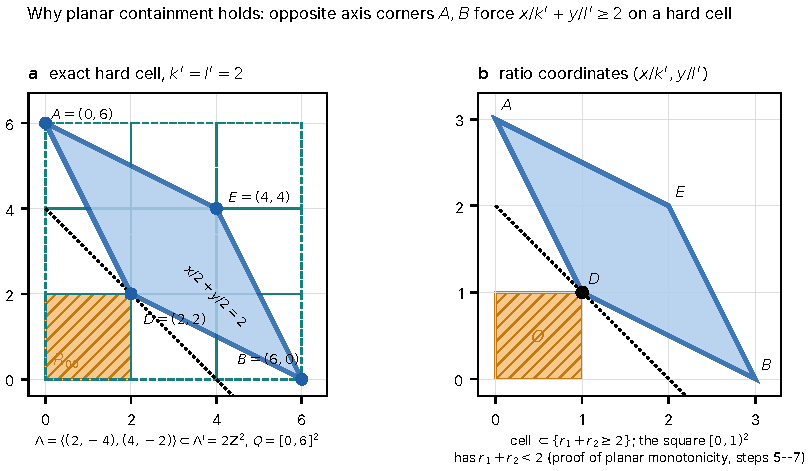
\includegraphics[width=0.98\textwidth]{fig08_planar_proof}
\caption{Geometry of the planar proof (\cref{thm:planar}, steps (1)--(7); \emph{exact computation of one instance of the construction}). Hard cell $c=\Pil((0,6);(2,-4),(4,-2))$ of the source lattice $\{x+2y\equiv0,\ 2x+y\equiv0\ (6)\}$, target $\Lambda'=2\Z^2$ (so $k'=l'=2$), box $[0,6]^2$. (a)~Opposite axis corners $A=(0,6)$ and $B=(6,0)$ and the other two corners $D=(2,2)$, $E=(4,4)$; the dotted line $x/k'+y/l'=2$ (i.e.\ $x+y=4$) passes through $D$, the corners $A,B,E$ lie strictly above it, and the whole cell lies on or above it; the $2\times2$ rectangles of the target tiling of $[0,x_0]\times[0,y_0]$ are dashed teal, and the corner square $[0,2]^2$ at the origin (orange, hatched) is the region the cell never enters. (b)~The same cell in the ratio coordinates $(x/k',y/l')$, where all four corners satisfy the inequality; by convexity so does every point of $c$. All $441$ grid points of $c$ were tested exactly against $U(2\Z^2,Q)$. The cell is an actual hard cell, not a schematic; the picture illustrates the general argument by this instance.}\label{fig:planarproof}
\end{figure}
\begin{remark}[why the plane works]\label{rem:whyplane}
In the proof the cell escapes only through the origin, and the escape is blocked by a fact that is special to $k=2$: opposite axis corners $A=(0,y_0)$, $B=(x_0,0)$ force every point of the cell to satisfy $x/k'+y/l'\ge2$, and for two ratios ``sum $\ge2$'' implies ``one ratio $\ge1$''. For three ratios a sum of $2$ is compatible with all ratios $<1$: in \cref{thm:C1} the failing cell has all four corners at ratio sum exactly $2$ (with axis orders $(2,2,2)$), and its point $(\tfrac23,\tfrac53,\tfrac53)$ has ratios $(\tfrac13,\tfrac56,\tfrac56)$, all $<1$. This explains where the planar argument cannot be repeated; it is not by itself a theorem about dimension three, and the failures proved in \cref{sec:obstruction} do not depend on it.
\end{remark}
\begin{corollary}[earlier planar conjectures]\label{cor:CP}
Conjecture CP2 (planar containment for $\Lambda\subsetneq\Lambda'$, same primes and box) and conjecture CP3-A (residual planar containment) of the earlier releases are theorems for nested lattices: they are \cref{thm:planar}. Both records remain in the crosswalk with their historical status OPEN; they are not restated.
\end{corollary}
\prov{CW-0473}{CP2}{OPEN}{EXCLUDED}
\prov{CW-0482}{CP3-A}{OPEN}{EXCLUDED}

\subsection{Relation to the inherited planar stabilisation theorem}\label{sec:g12}
GEO-I (v004 S1, cited as \texttt{CW-0477}) reduces every planar lattice $\Lambda_b$ to a normal form $\mathrm{diag}(a,c)\,\Gamma_{d,s}$ with $\Gamma_{d,s}=\{(i,j):j\equiv si\ (\mathrm{mod}\ d)\}$, $s$ a unit, and box $(\lfloor q_1/a\rfloor,\lfloor q_2/c\rfloor)$. The inherited theorem G12-T8 (GEO-I v012; cited as \texttt{CW-0478}, not reproved) states: for $d\ge2$, normalised box $\ge(d,d)$ and $\ne(d,d)$ one has $U=\conv F$. In that regime $U\subseteq U'$ follows from $F\subseteq F'$ by \cref{lem:gap} with no hypothesis on the lattices. \Cref{thm:planar} complements this: it needs $\Lambda\subseteq\Lambda'$ but holds for \emph{every} box, including the exceptional hollow box $(d,d)$ and sub-threshold boxes, where $U\ne\conv F$. The planar hole creation and destruction of \cref{prop:topology} occurs exactly at those exceptional boxes (ER-19).
\prov{CW-0477}{P3-L1}{PROVED}{CITED}
\prov{CW-0478}{P3-C1}{PROVED}{CITED}

\subsection{Scope for collective transitions}\label{sec:p5p1a}
\begin{proposition}[scope of the FIELD-I corollary (ER-23)]\label{prop:scope}
Let $x\to\Cmap(x)$ be an admissible planar transition ($k=2$, same primes and box). Then $U(\Lambda_x,Q)\subseteq U(\Lambda_{\Cmap(x)},Q)$ \emph{provided} $\Lambda_x\subseteq\Lambda_{\Cmap(x)}$. The collective map guarantees only $F\subseteq F'$, and lattices that shrink or are incomparable do occur (\cref{prop:corpus}), so \cref{thm:planar} does not by itself settle every planar transition.
\end{proposition}
\prov{CW-0505}{P5-P1.a}{PROVED}{FULL}
\begin{proof}
The first sentence is \cref{thm:planar}; the rest restates \cref{prop:fibre-vs-lattice}(b) and \cref{prop:corpus}. \qedhere
\end{proof}
For a transition with $F\subseteq F'$ but incomparable lattices, containment of the unions is not established in this manuscript.

\section{Dimension three: obstruction to preservation}\label{sec:obstruction}
For $k=3$ the inclusion $\Lambda\subseteq\Lambda'$ no longer implies $U(\Lambda,Q)\subseteq U(\Lambda',Q)$. \Cref{thm:evensum} already gives an infinite family with rectangular target $\bigoplus o_i\Z$. This section shows that the failure does not depend on the target having a coordinate on which it is ``free'', and gives the exact structure of the failing cells.

\subsection{Dilation invariance}
\begin{theorem}[diagonal dilation]\label{thm:D1}
Let $D=\mathrm{diag}(t_1,\dots,t_k)$ with $t_i$ positive integers and $M$ a lattice. Then $\Gr(DM)=D\,\Gr(M)$, $F(DM,DQ)=D\,F(M,Q)$, cells go to cells, $U(D\Lambda,DQ)=D\,U(\Lambda,Q)$, and
\[
U(\Lambda,Q)\subseteq U(\Lambda',Q)\iff U(D\Lambda,DQ)\subseteq U(D\Lambda',DQ).
\]
\end{theorem}
\prov{CW-0507}{P5-D1}{PROVED}{FULL}
\begin{proof}
$D:M\to DM$ is a bijection of lattices and $Dw\cm Dv\iff w\cm v$ (signs agree and $|t_iw_i|\le|t_iv_i|\iff|w_i|\le|v_i|$), so $D$ preserves the conformal order, hence Graver sets, independence, and the corner condition; it maps $M\cap[0,Q]$ onto $DM\cap[0,DQ]$ and $0$ to $0$. Cells are affine images of cubes. \qedhere
\end{proof}
Dilation changes the axis orders: the property ``$e_c\notin\Lambda'$'' is not dilation invariant, and a failure with a free coordinate becomes a failure in which every axis order is $\ge2$.

\subsection{A failure without free coordinate, and its dilation family}
\begin{theorem}[failure with no free coordinate]\label{thm:C1}
Let $E_3=\{z\in\Z^3:\sum z_i\text{ even}\}$, $\Lambda=2E_3\subseteq\Lambda'=2\Z^3$ (axis orders $(2,2,2)$: no $e_i$ lies in $\Lambda'$) and $Q=(2,4,2)$. Then $U(\Lambda,Q)\not\subseteq U(\Lambda',Q)$.
\end{theorem}
\prov{CW-0508}{P5-C1}{PROVED}{FULL}
\begin{proof}
$\Gr(2E_3)=2\,\Gr(E_3)$ (\cref{thm:D1} and \cref{prop:E25}). Let $g=(0,2,-2)=2(0,1,-1)$, $h=(2,-2,0)=2(1,-1,0)$, $u=(0,2,2)$. The corners $(0,2,2),(0,4,0),(2,0,2),(2,2,0)$ are nonzero points of $2E_3\cap Q$, so $c=\Pil(u;g,h)$ is a $2$-cell of $U(\Lambda,Q)$. The point $p=u+\tfrac16g+\tfrac13h=(\tfrac23,\tfrac53,\tfrac53)$ lies in $c$. In $U(2\Z^3,Q)$ the Graver vectors are $\pm2e_i$, so every cell is $\Pil(c';2e_i,i\in I)$ with $c'\in2\Z^3$. A cell containing $p$ must, for each coordinate $i$ with $0<p_i<2$ (all three do), use the generator $2e_i$ with base coordinate $0$; that cell is $[0,2]^3$, whose corner $0$ is excluded. So $p\notin U(\Lambda',Q)$. \qedhere
\end{proof}
\begin{figure}[tbp]\centering
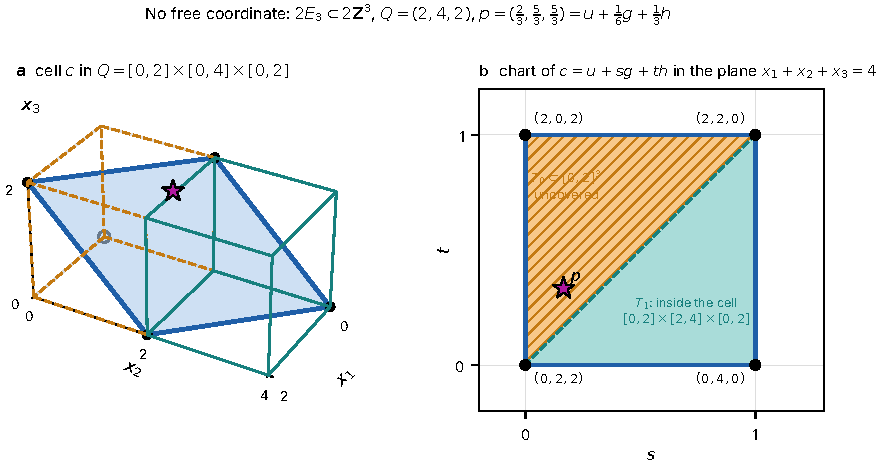
\includegraphics[width=0.98\textwidth]{fig09_noncontainment_3d}
\caption{Three-dimensional non-containment (\cref{thm:C1}; $\Lambda=2E_3\subset\Lambda'=2\Z^3$, $Q=(2,4,2)$; \emph{exact computation}). (a)~The $2$-cell $c=\Pil((0,2,2);(0,2,-2),(2,-2,0))$ of $\Kabs(2E_3,Q)$ in the box $[0,2]\times[0,4]\times[0,2]$ with its four corners $(0,2,2)$, $(0,4,0)$, $(2,0,2)$, $(2,2,0)$. (b)~The chart $c=u+sg+th$, $(s,t)\in[0,1]^2$, in the plane $x_1+x_2+x_3=4$: the part $T_0$ of $c$ inside the cube $[0,2]^3$ (light orange) is not covered by any cell of $\Kabs(2\Z^3,Q)$, whereas the part $T_1$ (outside that cube) is. The star is the witness $p=(\frac23,\frac53,\frac53)=u+\frac16g+\frac13h\in T_0$, in $c$ but in no cell of $\Kabs(2\Z^3,Q)$ (exact enumeration); hence $U(2E_3,Q)\not\subseteq U(2\Z^3,Q)$.}\label{fig:noncontain}
\end{figure}
\begin{corollary}[infinite family]\label{cor:C2}
If $(\Lambda,\Lambda',Q)$ fails (i.e.\ $U(\Lambda,Q)\not\subseteq U(\Lambda',Q)$) then so does every dilation $(D\Lambda,D\Lambda',DQ)$. In particular every failing triple with a free coordinate, such as the scaled $E_3\subset\Z^3$, $Q=(1,2,1)$, $p=(\tfrac13,\tfrac56,\tfrac56)$, generates failing triples all of whose axis orders are $\ge2$.
\end{corollary}
\prov{CW-0509}{P5-C2}{PROVED}{FULL}
\begin{proof}
\Cref{thm:D1}. \qedhere
\end{proof}
\begin{figure}[tbp]\centering
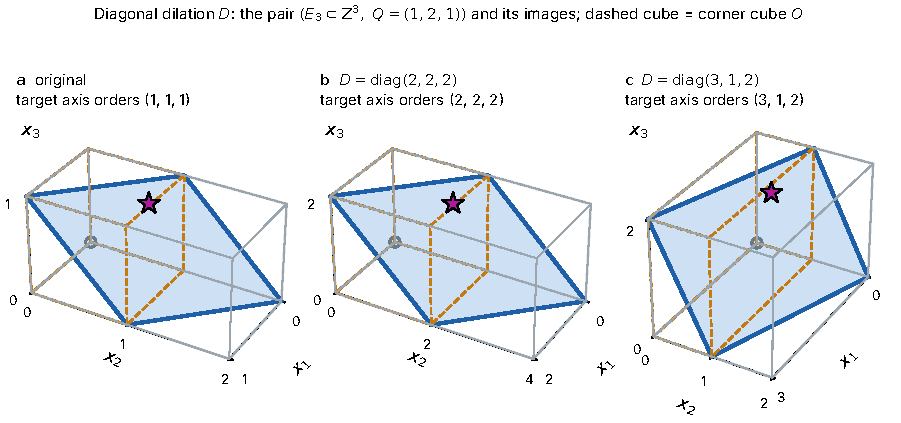
\includegraphics[width=0.98\textwidth]{fig10_dilation}
\caption{Diagonal dilation preserves failure (\cref{thm:D1,cor:C2}; \emph{exact computation}). The failing pair $(E_3\subset\Z^3,Q=(1,2,1))$ with its witness $(\frac13,\frac56,\frac56)$ (a) and two dilations: $D=\mathrm{diag}(2,2,2)$ giving $(2E_3\subset2\Z^3,(2,4,2))$ with witness $(\frac23,\frac53,\frac53)$ (b) --- the configuration of \cref{fig:noncontain} --- and $D=\mathrm{diag}(3,1,2)$ giving the box $(3,2,2)$ with witness $(1,\frac56,\frac53)$ (c). In each panel the transformed box, the cell and the transformed corner cube (dashed) are drawn; the target axis orders are $(1,1,1)$, $(2,2,2)$ and $(3,1,2)$, so in (a) every coordinate is free, in (b) none is, and in (c) only $x_2$ is. Failure was verified exactly in all three cases.}\label{fig:dilation}
\end{figure}
\begin{remark}[relation to the corner-cube theorem]
Theorem~\ref{thm:C1} is the instance $o=(2,2,2)$ of \cref{thm:evensum}: the scaled source lattice is $E_3$, the scaled box is $(1,2,1)$ with maximum $2$, and the scaled point is $(\tfrac13,\tfrac56,\tfrac56)\in O$. The target $2\Z^3$ is rectangular in the sense of \cref{sec:corner}; the release derived the same example independently and emphasises ``no free coordinate'' because the earlier three-dimensional conjecture was formulated in those terms. (The identification is derived here from the two cited theorems and the scaling invariance; it is an elementary observation.) The recorded $57$ lattice-level failures with a free coordinate are finite-exact data of the releases and are not used.
\end{remark}

\subsection{A target that is not split in any coordinate}
\begin{proposition}[FINITE-EXACT; body-centred target]\label{prop:C3}
Let $\Lambda=2E_3$, $\Lambda'=\mathrm{BCC}=\{z\in\Z^3:z_1\equiv z_2\equiv z_3\ (2)\}$ (index $4$, axis orders $(2,2,2)$, not split in any coordinate: $\Lambda'\ne(\Lambda'\cap\{z_i=0\})\oplus(\Lambda'\cap\R e_i)$ for each $i$) and $Q=(2,4,2)$. Then $\Lambda\subseteq\Lambda'$ and $U(\Lambda,Q)\not\subseteq U(\Lambda',Q)$; the cell $c$ of \cref{thm:C1} contains the point $(\tfrac56,\tfrac53,\tfrac32)=u+\tfrac14g+\tfrac5{12}h$, which is not in $U(\mathrm{BCC},Q)$. The same source cell is contained in $U(E_3,Q)$ (release; also sampled at $49$ interior points here).
\end{proposition}
\prov{CW-0510}{P5-C3}{FINITE-EXACT}{FINITE}
\noindent\emph{Evidence and scope.} The statement is a finite exact computation: for $Q=(2,4,2)$, $\Kabs(\mathrm{BCC},Q)$ has $13$ vertices, $33$ edges, $17$ squares and one cube, and the point lies in no cell. The release certified this by three routes (an engine with an independent certificate checker, a mini brute-force implementation, and the preregistered pinned engine); it was reproduced here with a fourth, independent exact implementation (\texttt{scripts/run\_exact\_checks.py}). Non-splitness of BCC: for each $i$, $\Lambda'\cap\{z_i=0\}=2\Z^2$ and $\Lambda'\cap\R e_i=2\Z e_i$, whose direct sum has index $8$ in $\Z^3$, while $[\Z^3:\Lambda']=4$; so $\Lambda'$ is not that direct sum. The release also records failure for $\Lambda'=E_2\times2\Z$ (split in one coordinate), cited. \textbf{Consequence:} neither ``no free coordinate'' nor even ``no split coordinate'' implies preservation; the $3$-dimensional conjecture of the earlier assessment ($\Lambda\subseteq\Lambda'\subseteq\Z^3$, $e_1,e_2,e_3\notin\Lambda'\Rightarrow U\subseteq U'$) is false, by \cref{thm:C1} already.

\begin{figure}[tbp]\centering
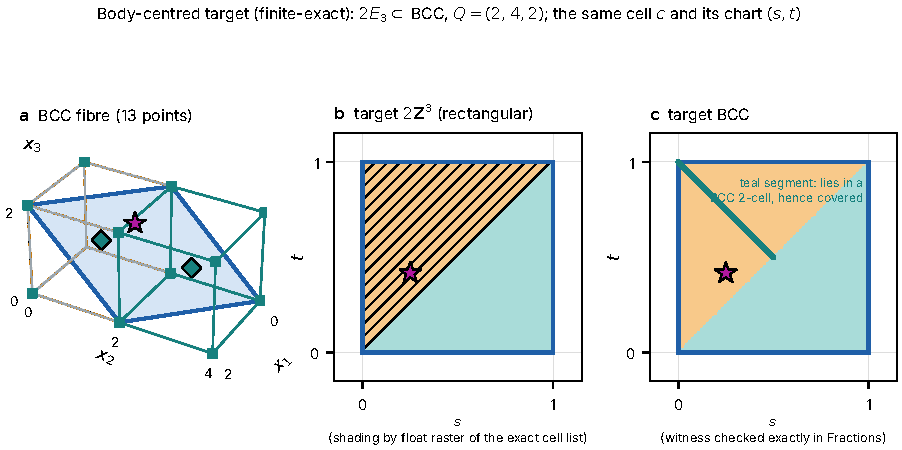
\includegraphics[width=0.98\textwidth]{fig11_bcc}
\caption{The body-centred target (\cref{prop:C3}; FINITE-EXACT for $Q=(2,4,2)$ only). The cell $c$ of \cref{fig:noncontain} and its chart $(s,t)$. (a)~The $13$ points of $F(\mathrm{BCC},Q)$, $\mathrm{BCC}=\{z_1\equiv z_2\equiv z_3\ (2)\}$. (b)~With the rectangular target $2\Z^3$ ($f$-vector $(11,17,8,1)$) the uncovered region is the orange triangle $T_0$ of \cref{fig:noncontain}. (c)~With the BCC target ($f$-vector $(13,33,17,1)$) the uncovered region is $T_0$ minus a teal segment, which lies in a BCC $2$-cell and is therefore covered; but the exact witness $p=(\frac56,\frac53,\frac32)$ (chart coordinates $(\frac14,\frac5{12})$, star) lies in no cell of $\Kabs(\mathrm{BCC},Q)$. Shading is a floating-point raster (uncovered fractions $\approx0.497$ and $\approx0.493$ of the chart); the verdict at $p$ is exact. This is a finite-exact example, not a classification of non-split targets.}\label{fig:bcc}
\end{figure}
\subsection{Cells inside a coordinate plane are preserved}
\begin{theorem}\label{thm:F1}
Let $\Lambda\subseteq\Lambda'\subseteq\Z^3$ and let $c$ be a cell of $U(\Lambda,Q)$ contained in a coordinate plane $H=\{x_i=0\}$. Then $c\subseteq U(\Lambda',Q)$. So a failing cell is never in a coordinate plane.
\end{theorem}
\prov{CW-0506}{P5-F1}{PROVED}{FULL}
\begin{proof}
A vector conformally below one in $H$ lies in $H$, so $\Gr(M\cap H)=\Gr(M)\cap H$ for every lattice $M$. Hence $c$ is a cell of the planar pair $\Lambda\cap H\subseteq\Lambda'\cap H$ (both of rank $2$), and \cref{thm:planar} gives $c\subseteq U(\Lambda'\cap H,Q\cap H)$. Cells of $\Lambda'\cap H$ with corners in $F(\Lambda'\cap H)$ are cells of $\Lambda'$ (their generators are Graver in $\Lambda'$ by the same identity), so $U(\Lambda'\cap H,Q\cap H)\subseteq U(\Lambda',Q)$. \qedhere
\end{proof}

\subsection{Finite census (finite-exact)}
\begin{proposition}[FINITE-EXACT; scope as stated]\label{prop:census}
Targets of index $2$--$6$ without a free coordinate ($96$ lattices), sources of index $2$--$5$ ($8{,}256$ pairs), all hard cells with bounding box $\le Q_{\max}=(\min(3k_c,12))_c$: $24{,}178$ hard cells ($6{,}825$ squares, $17{,}353$ cubes), each tested against its own worst box. $192$ hard cells fail; the failing targets are $19$ of the $96$: all $12$ split targets and $7$ of $84$ non-split targets (BCC and six of index $6$). The remaining $77$ non-split targets (including $E_3$ and every target of index $3$ and $5$) have no failure among $19{,}794$ hard cells. An extended run (sources of index $6$--$9$ in the $18$ clean targets of index $\le4$) found $19{,}877$ hard cells and no failure.
\end{proposition}
\prov{CW-0512}{census}{FINITE-EXACT}{FINITE}
\noindent These numbers are samples, not a classification theorem, and the release states explicitly that its earlier remark ``no zero-vertex decomposition occurred'' was an artefact of box scope. They are included only to indicate that preservation for non-split targets is genuinely dependent on the target lattice; the question of which non-split targets preserve $U$ is open (\cref{sec:open}).

\section{Slabs: split targets and the corrected criterion}\label{sec:slab}
Suppose the target splits along the third coordinate with period $k$: $\Lambda'=\Lambda'_2\oplus k\Z e_3$, with $\Lambda'_2$ a rank-two lattice in the $(x_1,x_2)$-plane. (The symbol $k$ is the period here, not the dimension.) For $k=1$ the coordinate is \emph{free} ($e_3\in\Lambda'$). Write $Q=(Q',q_3)$, $J=\lfloor q_3/k\rfloor$, $U=U(\Lambda'_2,Q')$ and $U^0=U^0(\Lambda'_2,Q')$ (planar, origin excluded, resp.\ allowed). The three-dimensional union is a stack of planar unions with a single exceptional layer.

\subsection{The union of a split target}
\begin{theorem}[slab structure]\label{thm:slab-i}
For $J\ge1$, $U(\Lambda',Q)=\bigl[U\times[0,k]\bigr]\cup\bigl[U^0\times[k,kJ]\bigr]$; for $J=0$, $U(\Lambda',Q)=U\times\{0\}$.
\end{theorem}
\prov{CW-0511}{P5-S4}{PROVED}{FULL}
\begin{proof}
A nonzero vector $(a,t)$ of $\Lambda'$ with $a\ne0\ne t$ has $(a,0)\in\Lambda'$ conformally below it, so it is not Graver; $(a,0)$ is Graver in $\Lambda'$ iff $a$ is Graver in $\Lambda'_2$; $(0,t)$ is Graver iff $|t|=k$. So $\Gr(\Lambda')=\{(g,0):g\in\Gr(\Lambda'_2)\}\cup\{\pm ke_3\}$ and every cell of $\Lambda'$ is $c_2\times\{z\}$ or $c_2\times[z,z+k]$ with $c_2$ a planar cell (generators in $\Gr(\Lambda'_2)$), $z\in k\Z$, $z\ge0$ (and $z+k\le q_3$ in the second case). The corner $(v,z)$ is zero iff $v=0$ and $z=0$. For $z=0$ the planar factor must avoid the corner $0$: $c_2$ is a cell of $U$; for $z\ge k$ the origin is allowed: $c_2$ is a cell of $U^0$. In the second form the corners with third coordinate $z+k\ge k$ impose nothing more. Taking the union over $z$: heights in $[0,k]$ are covered by cells with $z=0$ (giving $U$ at heights $<k$) and heights in $[k,kJ]$ by cells with $z\ge k$ (giving $U^0$); at height exactly $k$ both occur and $U\subseteq U^0$. For $J=0$ only $z=0$ and no $\pm ke_3$ exist. \qedhere
\end{proof}
\begin{corollary}[free coordinate: slab lemma]\label{cor:slab-lemma}
If $e_3\in\Lambda'$ ($k=1$) and $q_3\ge1$ then for $0<c<1$: $(x',c)\in U(\Lambda',Q)\iff x'\in U(\Lambda'_2,Q')$; and for $c\in[1,q_3]$ the slice is $U^0$. If a point $p\in U(\Lambda,Q)$ has $0<p_3<1$ and its planar part lies outside $U(\Lambda'_2,Q')$, then $U(\Lambda,Q)\not\subseteq U(\Lambda',Q)$ (slab obstruction).
\end{corollary}
\prov{CW-0492}{P4-S1}{PROVED}{FULL}
\prov{CW-0494}{P4-S2}{PROVED}{ADAPTED}
\begin{proof}
\Cref{thm:slab-i} with $k=1$. \qedhere
\end{proof}
The slab lemma shows that a free-coordinate obstruction is inherited from the planar target: a planar gap times a thin slab. It is not a new three-dimensional coupling.

\subsection{The corrected containment criterion}\label{sec:slab-ii}
\begin{theorem}[containment criterion, corrected form]\label{thm:slab-ii}
Let $\Lambda\subseteq\Lambda'=\Lambda'_2\oplus k\Z e_3$ and let $c$ be a cell of $U(\Lambda,Q)$. Then
\[
c\subseteq U(\Lambda',Q)\iff\Bigl[\ \min_{x\in c}x_3\ge k\ \Bigr]\ \text{ or }\ \Bigl[\ \mathrm{proj}_{12}\bigl(c\cap\{x_3\le k\}\bigr)\subseteq U(\Lambda'_2,Q')\ \Bigr].
\]
Equivalently: $c\subseteq U(\Lambda',Q)$ iff $\mathrm{proj}_{12}(c\cap\{x_3<k\})\subseteq U$.
\end{theorem}
\prov{CW-0511}{P5-S4(ii)'}{PROVED}{FULL}
\begin{proof}
The corners of $c$ lie in $\Lambda\subseteq\Lambda'$, so their third coordinates lie in $k\Z\cap[0,q_3]$, and $c\subseteq\{0\le x_3\le kJ\}$. By \cref{thm:slab-i} the slice of $U(\Lambda',Q)$ at height $z<k$ is $U$ and at height $z\in[k,kJ]$ is $U^0$ (for $J=0$ the cell lies in $\{x_3=0\}$ and the slice is $U$). Hence $c\subseteq U(\Lambda',Q)$ iff (a) $\mathrm{proj}_{12}(c\cap\{x_3<k\})\subseteq U$ and (b) $\mathrm{proj}_{12}(c\cap\{k\le x_3\le kJ\})\subseteq U^0$.

\emph{Claim: (b) always holds, indeed $\mathrm{proj}_{12}(c)\subseteq U^0$.} The projection of $c=\Pil(u;g_1,\dots,g_j)$ is the zonogon $\mathrm{proj}(u)+\sum[0,1]\mathrm{proj}(g_l)$ where $\mathrm{proj}(g_l)\in\Lambda'_2$ (the projection maps $\Lambda'$ into $\Lambda'_2$); its corners are projections of corners of $c$, hence lie in $\Lambda'_2\cap Q'$ (the origin allowed). Decompose each $\mathrm{proj}(g_l)$ by \cref{lem:L1} into Graver vectors of $\Lambda'_2$ conformally below it and tile the zonogon by \cref{lem:T0}. As in the proof of \cref{prop:Z} (Z.1), every tile vertex is the sum of the base and partial sums of the pieces; its coordinates lie between coordinates of corners of the projected cell, hence in $[0,Q']$, and it lies in $\Lambda'_2$. With the origin allowed, every tile is a cell of $U^0$, so $\mathrm{proj}(c)\subseteq U^0$.

Therefore $c\subseteq U(\Lambda',Q)$ iff (a). If $c\cap\{x_3<k\}=\emptyset$ (that is $\min x_3\ge k$) (a) is vacuous. Otherwise $c\cap\{x_3<k\}$ is a nonempty convex subset of the convex set $c$ whose closure is $c\cap\{x_3\le k\}$ (move from any point of $c\cap\{x_3\le k\}$ towards a point with $x_3<k$); since $U$ is closed and the projection is continuous, (a) is equivalent to $\mathrm{proj}(c\cap\{x_3\le k\})\subseteq U$. \qedhere
\end{proof}
\begin{remark}[the erratum]\label{rem:E1}
The first release of this criterion (v005, P5-S4(ii)) stated the condition $\mathrm{proj}_{12}(c\cap\{x_3\le k\})\subseteq U$ \emph{without} the alternative $\min x_3\ge k$. That closed-height form is false, and it is \emph{not} stated as valid here. Counterexample (erratum E1, ER-22, reproduced independently here): $\Lambda=2\Z^2\oplus2\Z$, $\Lambda'=\Z^2\oplus2\Z$ (period $k=2$), $Q=(2,2,2)$, $c=[0,2]^2\times\{2\}=\Pil((0,0,2);(2,0,0),(0,2,0))$. Then $c$ is a source cell and $c\subseteq U(\Lambda',Q)$ (for instance $(\tfrac12,\tfrac12,2)\in U(\Lambda',Q)$ because at height $2=k$ the target already contains the vertex $(0,0,2)\ne0$, so its slice there is $U^0$, not $U$); but the closed-height criterion would reject $c$ because $(\tfrac12,\tfrac12)\notin U(\Z^2,(2,2))$. All earlier consequences of the \emph{hard-cell} comparisons were unaffected: a hard cell has $\min x_3=0<k$, where the closed form is correct.
\end{remark}

\begin{figure}[tbp]\centering
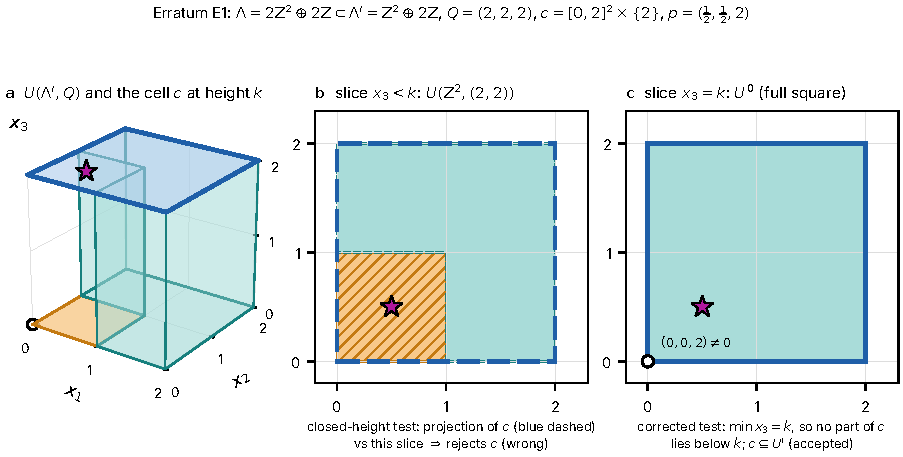
\includegraphics[width=0.98\textwidth]{fig13_strict_slab}
\caption{Why the strict-slab correction matters (\cref{thm:slab-ii}, \cref{rem:E1}; $\Lambda=2\Z^2\oplus2\Z\subset\Lambda'=\Z^2\oplus2\Z$, $k=2$, $Q=(2,2,2)$; \emph{exact computation}). The cell $c=[0,2]^2\times\{2\}$ lies at height $x_3=k$. (a)~$U(\Lambda',Q)$ and $c$. (b)~The slice $x_3<k$ is the origin-excluded $U(\Z^2,(2,2))$, which does not contain $(\frac12,\frac12)$. (c)~The slice $x_3=k$ is the origin-allowed full square $U^0$. The point $p=(\frac12,\frac12,2)$ lies in $U(\Lambda',Q)$ (and all $121$ grid points of $c$ do), so $c\subseteq U(\Lambda',Q)$ and the corrected criterion (strict height $x_3<k$; here $c\cap\{x_3<k\}=\emptyset$) accepts $c$. The closed-height form of the first release would require $\mathrm{proj}_{12}(c)\subseteq U(\Z^2,(2,2))$, which fails at $(\frac12,\frac12)$, and would wrongly reject $c$.}\label{fig:strict}
\end{figure}
\subsection{The free-coordinate case}
\begin{corollary}[complete slab criterion]\label{cor:S3}
Let $e_3\in\Lambda'$ ($k=1$), $q_3\ge1$ and $\Lambda\subseteq\Lambda'$. Then $U(\Lambda,Q)\subseteq U(\Lambda',Q)$ iff there is no point $p\in U(\Lambda,Q)$ with $p_3<1$ whose planar part lies outside $U(\Lambda'_2,Q')$.
\end{corollary}
\prov{CW-0498}{P4-S3}{PROVED}{ADAPTED}
\begin{proof}
\Cref{thm:slab-ii} with $k=1$, applied to every cell: $c\subseteq U'$ iff $\mathrm{proj}(c\cap\{x_3<1\})\subseteq U$. \qedhere
\end{proof}
In particular, for free-coordinate targets every failure is a slab obstruction (the ``S1 failures'' of the intermediate releases do not exist), and the failures of this class are exactly the planar target gaps seen through the layer $0<x_3<1$. The slab criterion is drawn in \cref{fig:slab}.
\begin{figure}[tbp]\centering
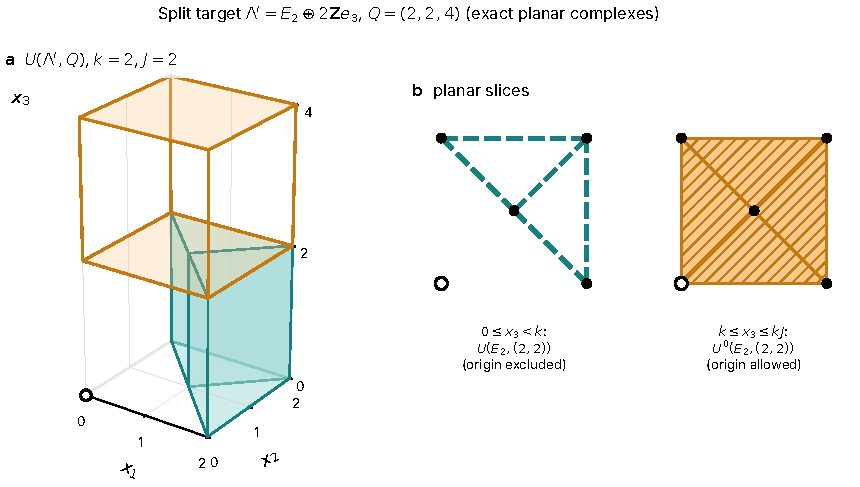
\includegraphics[width=0.98\textwidth]{fig12_slab_structure}
\caption{Geometry of a split target (\cref{thm:slab-i}; $\Lambda'=E_2\oplus2\Z e_3$, $Q=(2,2,4)$, $k=2$, $J=2$; planar complexes \emph{exact}, vertical stacking \emph{schematic}). (a)~The union $U(\Lambda',Q)$: below height $k$ the slice is the origin-excluded planar union $U=U(E_2,(2,2))$ (blue; one-dimensional here, $5$ edges and no square), from height $k$ upward it is the origin-allowed union $U^0$ (orange; the filled square $[0,2]^2$ and $8$ edges). (b)~The two planar slices. A source cell is contained iff its part below height $k$ projects into $U$. The figure shows a realised union, not an abstract complex.}\label{fig:slab}
\end{figure}

\section{Hard cells and a coupled-target specimen}\label{sec:hard}

\subsection{Structure of a hard cell}
\begin{proposition}[a hard cell is a Minkowski sum of segments]\label{prop:H1}
Let $\Lambda\subseteq\Lambda'$ and let $c=\Pil(u;g_1,\dots,g_j)$ be a hard cell of $U(\Lambda,Q)$ in the sense of \cref{prop:Z}. Put $a_i=-g_i^-\ge0$ and $b_i=g_i^+\ge0$; both lie in $\Lambda'$, have disjoint supports and $g_i=b_i-a_i$. Then $u=\sum a_i$ and
\[
\begin{gathered}c=\sum_i[a_i,b_i]\ \subseteq\ Z^0:=\sum_i\bigl([0,a_i]+[0,b_i]\bigr)\ \subseteq\ [0,Q_c],\\ Q_c=\sum_i(a_i+b_i)\ \text{(the top corner of $c$)}.\end{gathered}
\]
In a fine tiling of $Z^0$ by Graver pieces of the $a_i,b_i$ (\cref{lem:L1,lem:T0}) every tile that does not contain the origin as a vertex is a cell of $U(\Lambda',Q_c)$; the origin is the only vertex that is not a nonzero subset sum. Hence the only part of $c$ that can fail to lie in $U(\Lambda',Q_c)$ is $c\cap\mathrm{St}(0)$, the star of the origin in the tiling.
\end{proposition}
\prov{CW-0503}{E2P4v5-H1}{PROVED}{FULL}
\begin{proof}
$m(c)=u+\sum g_i^-=0$ gives $u=\sum a_i$, and $u+\sum\lambda_ig_i=\sum_i[(1-\lambda_i)a_i+\lambda_ib_i]$, which is a point of $\sum[a_i,b_i]\subseteq Z^0$. The pieces of the $a_i,b_i$ are nonnegative nonzero vectors, so a subset sum vanishes only for the empty subset; the vertices of tiles of $Z^0$ are subset sums and the remaining argument is that of \cref{prop:Z}(Z.1) with $s_i$ the partial sums. Coordinates stay in $[0,Q_c]$ because all pieces are $\ge0$. \qedhere
\end{proof}
This is the precise form of the statement ``the deleted origin matters only for cells that touch every coordinate plane''. In the plane the star of the origin is covered by the coarser rectangular tiling (the proof of \cref{thm:planar}); in the examples of \cref{sec:obstruction} the star of the origin is the corner cube.

\begin{figure}[tbp]\centering
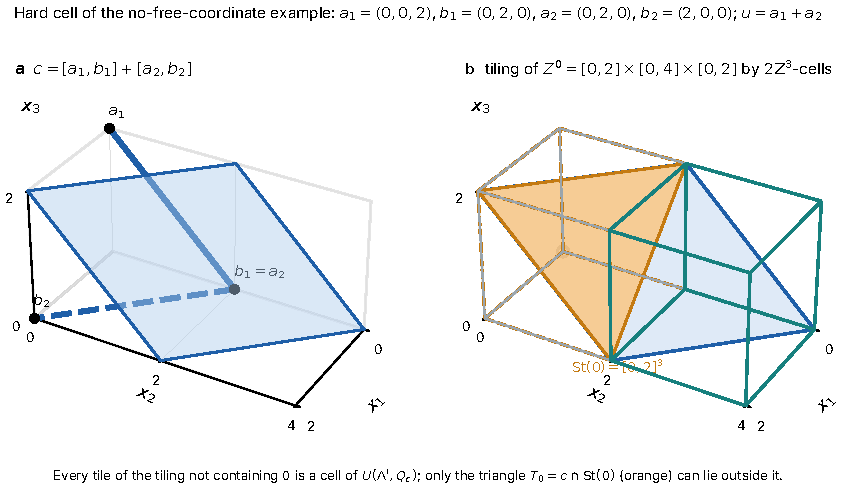
\includegraphics[width=0.98\textwidth]{fig14_hard_cell}
\caption{Minkowski decomposition of a hard cell and the origin star (\cref{prop:H1}; the cell $c$ of \cref{thm:C1}, $\Lambda=2E_3$, $\Lambda'=2\Z^3$; \emph{exact computation}). (a)~$c=[a_1,b_1]+[a_2,b_2]$ with $a_1=(0,0,2)$, $b_1=(0,2,0)$, $a_2=(0,2,0)$, $b_2=(2,0,0)$ and $u=a_1+a_2=(0,2,2)$, drawn as the sum of two segments. (b)~The zonotope $Z^0=[0,2]\times[0,4]\times[0,2]$ tiled by $2\Z^3$-cells: the tile $[0,2]^3$ has the origin as a vertex and is the star $\mathrm{St}(0)$ (orange; it is not a cell of $\Kabs(2\Z^3,Q)$ because the origin is not in the fibre), the tile $[0,2]\times[2,4]\times[0,2]$ is a cell of the target. The only part of $c$ not covered by non-star tiles lies in $\mathrm{St}(0)$; this is the region $T_0$ of \cref{fig:noncontain}.}\label{fig:hardcell}
\end{figure}
\subsection{The coupled specimen P4-F110}
The previous sections concern general lattices. We record the one explicit coupled collective transition for which the whole transport can be decided for every box size $m$.
\begin{proposition}[arithmetic of P4-F110]\label{prop:P4A}
For every integer $m\ge1$, $x_m=2\cdot110^{4m}/9$ has $L=110^{2m}$, $G=9$, $\Cmap(x_m)=110^{4m}/3=:y_m$; the active primes $(2,5,11)$ and the box $Q_m=[0,2m]^3$ are the same for $x_m$ and $y_m$. The relation lattices are $\Lambda_9=\{(a,b,c):a-b+c\equiv0\ (6)\}$ and $\Lambda_3=E_3$, with $\Lambda_9\subsetneq\Lambda_3$; the orders modulo $9$ are $(6,6,6)$ and modulo $3$ are $(2,2,2)$, and both lattices are non-rectangular.
\end{proposition}
\prov{CW-0483}{P4-A}{PROVED}{FULL}
\prov{CW-0484}{P4-L}{PROVED}{FULL}
\begin{proof}
$\mathrm{num}(x_m)=2^{4m+1}5^{4m}11^{4m}$, so $d^2\mid\mathrm{num}$ iff $d=2^a5^b11^c$ with $a,b,c\le2m$. Modulo $9$: $5\equiv2^{-1}$, $11\equiv2$, $\ord_9(2)=6$, so $d\equiv2^{a-b+c}$ and $d\equiv1$ iff $a-b+c\equiv0\ (6)$. Every $d\in D$ has $9\mid d-1$, so $9\mid G$. The vectors $(1,1,0)$ and $(0,1,1)$ give $10,55\in D$ with $\gcd(9,54)=9$, so $G=9$. The vectors $(2m,2m,0)$, $(0,2m,2m)$ give $10^{2m},55^{2m}\in D$, whose lcm is $110^{2m}$, and every $d\in D$ divides $110^{2m}$; so $L=110^{2m}$. Then $\Cmap(x_m)=(2+1)\cdot110^{4m}/9=110^{4m}/3$; the numerator $110^{4m}$ has $v_p=4m$ for $p=2,5,11$, so the primes and the box $[0,2m]^3$ are unchanged. Modulo $3$ all of $2,5,11$ are $-1$, so $\chi_3=(-1)^{a+b+c}$, and $a-b+c\equiv0\ (6)$ implies $a+b+c=(a-b+c)+2b$ even; $(2,0,0)\in E_3\setminus\Lambda_9$. \qedhere
\end{proof}
\begin{theorem}[hull theorem for $E_3$]\label{thm:hull}
Let $n\ge4$ be even and $Q=[0,n]^3$. Then $U(E_3,Q)=\conv F(E_3,Q)=\{z\in[0,n]^3:z_1+z_2+z_3\ge2\}$. For $n=2$ this fails.
\end{theorem}
\prov{CW-0485}{P4-T1}{PROVED}{ADAPTED}
\begin{proof}
(1) \emph{Hull.} $F$ contains all cube vertices except $0$ (their coordinate sums are even) and $(2,0,0),(0,2,0),(0,0,2)$, and every point of $F$ has coordinate sum $\ge2$. The polytope $[0,n]^3\cap\{\sum\ge2\}$ has exactly these $10$ vertices, so $\conv F$ equals it.
(2) \emph{Cube tiling.} $2e_i\in\Gr(E_3)$ (\cref{prop:E25}). For $w\in(2\Z)^3\cap[0,n-2]^3$, $w\ne0$, the eight corners $w+\{0,2\}^3$ have even sum, are nonzero and lie in the box, so the cube is a $3$-cell; these cubes tile $[0,n]^3$ minus the corner cube $[0,2]^3$.
(3) \emph{The corner cube.} We must show $[0,2]^3\cap\{\sum\ge2\}\subseteq U(E_3,[0,n]^3)$. The Graver set of $E_3$ in $[-n,n]^3$ is the same for every $n\ge2$ (a conformally minimal vector lies in the box of its own size) and $F(E_3,4)\subseteq F(E_3,n)$, so the cells of the box-$4$ complex are cells of the box-$n$ complex, and it suffices to take $n=4$. For $n=4$ the argument is a finite exact certificate, identified precisely in \cite{HD1P4}: the object \texttt{n4\_target\_hull\_cover} in \texttt{results/P4\_CERTIFICATES.json} of the release \texttt{GEO\_HD\_E2\_P4\_v001} (byte-identical in \texttt{v001}--\texttt{v004}), replayed by shard \texttt{S4} of that release. It is a decomposition of $\conv F(E_3,[0,4]^3)$ into pieces each lying in a single maximal cell of $\Kabs(E_3,[0,4]^3)$, with no gap nodes; it is a statement about one explicit polytope and one explicit finite set of cells. \emph{Logical role.} The certificate is used for exactly one implication: $[0,2]^3\cap\{\sum x_i\ge2\}\subseteq U(E_3,[0,4]^3)$, from which part~(3) follows for all even $n\ge4$ by the Graver-set argument above. Parts (1) and (2) do not use it. All of \cref{thm:hull}, and everything that cites it (\cref{thm:P4T2,cor:P4C1}), is therefore PROVED \emph{modulo this finite exact computation}, and this status is recorded in \cref{sec:open}. \emph{Independent replay.} Because the certificate is cited and not reproduced, the present manuscript supplies a separate exact check of the same implication (\texttt{scripts/replay\_n4\_cover.py}, output \texttt{results/N4\_COVER\_REPLAY.json}): in exact rational arithmetic it enumerates the $764$ three-dimensional cells of $\Kabs(E_3,[0,4]^3)$ and subtracts them from the polytope $[0,2]^3\cap\{\sum x_i\ge2\}$ by exact polytope subtraction; no piece remains. The same code applied to the box $[0,2]^3$ leaves $9$ pieces, the gap at $n=2$ (the release reports $94$ gap pieces for its own decomposition; piece counts depend on the decomposition used). This replay uses the cells of this manuscript's enumeration and is a manuscript-level check of the implication, not an independent verification of the release. As a further sanity check only, all $609$ points of the quarter-grid of $[0,2]^3$ with coordinate sum $\ge2$ lie in $U(E_3,[0,4]^3)$. For $n=2$ the statement fails: the point $(0,1,\tfrac32)$ lies in $\conv F$ (its sum is $\tfrac52\ge2$) but in no cell of $\Kabs(E_3,[0,2]^3)$ (exact enumeration here; the release certifies the gap at $n=2$ with $94$ gap pieces). This is consistent with the planar face $x_1=0$, where $E_3$ restricts to $E_2$ in the exceptional hollow box $(2,2)$. \qedhere
\end{proof}
\begin{theorem}[transport for P4-F110]\label{thm:P4T2}
For every $m\ge1$: $U(\Lambda_9,Q_m)\subsetneq U(E_3,Q_m)$, the transport class is ``source contained'', and $U(E_3,Q_m)\not\subseteq U(\Lambda_9,Q_m)$.
\end{theorem}
\prov{CW-0486}{P4-T2}{PROVED-SCOPED}{ADAPTED}
\begin{proof}
For $m\ge2$ ($n=2m\ge4$): $U(\Lambda_9)\subseteq\conv F(\Lambda_9)\subseteq\conv F(E_3)=U(E_3)$ by $F(\Lambda_9)\subseteq F(E_3)$ and \cref{thm:hull}. Strictness: $(2,0,0)$ is a vertex of $\conv F(E_3)$ lying in $F(E_3)$ but not in $F(\Lambda_9)$ ($2-0+0=2\not\equiv0\ (6)$); a vertex of $\conv F(E_3)$ that lies in $\conv F(\Lambda_9)\subseteq\conv F(E_3)$ is a vertex of $\conv F(\Lambda_9)$, hence in $F(\Lambda_9)$; so $(2,0,0)\notin U(\Lambda_9)$ (indeed $U(\Lambda_9)\subseteq\conv F(\Lambda_9)$). For $m=1$ ($n=2$, where \cref{thm:hull} fails) the release gives direct exact certificates (the two maximal source cells covered by $18$ target maximal cells, independently replayed); this finite certificate is cited. The reverse non-containment is the same vertex argument. \qedhere
\end{proof}
The scope of the theorem is the family P4-F110 only. A direct engine verification beyond $m=2$ was not attempted by the release (cost); the case $m\ge3$ is covered by \cref{thm:hull}.
\begin{corollary}[predictive criterion for $E_3$ targets]\label{cor:P4C1}
Let $\Lambda\subseteq E_3$ be any sublattice and $n\ge4$ even. Then $U(\Lambda,[0,n]^3)\subseteq U(E_3,[0,n]^3)$.
\end{corollary}
\prov{CW-0489}{P4-C1}{PROVED}{FULL}
\begin{proof}
$U(\Lambda)\subseteq\conv F(\Lambda)\subseteq\conv F(E_3)=U(E_3)$ by \cref{thm:hull}. \qedhere
\end{proof}
The first release of this result added an equality clause (equality of unions iff $\conv F(\Lambda)$ contains the ten vertices of \cref{thm:hull}); that clause is withdrawn (counterexample $\Lambda=2\Z^3$, $n=4$) and only the containment is stated (ER-21).
\prov{CW-0487}{P4-C1 (v001)}{CORRECTED}{EXCLUDED} Its predictive cost is $O(|F|)$ lattice-point tests with no cell reconstruction.
\begin{proposition}[holes are not obstructions; FINITE-EXACT, one specimen]\label{prop:holes}
For $m=1$ the target $E_3$ is not hull-covered (\cref{thm:hull}, $n=2$) and yet $U(\Lambda_9,Q_1)\subseteq U(E_3,Q_1)$.
\end{proposition}
\prov{CW-0488}{P4-O1}{FINITE-EXACT}{FINITE}
This is an observation about one specimen (the release certifies it exactly with $94$ gap pieces); it shows only that gaps of the target do not by themselves obstruct containment.
\begin{figure}[tbp]\centering
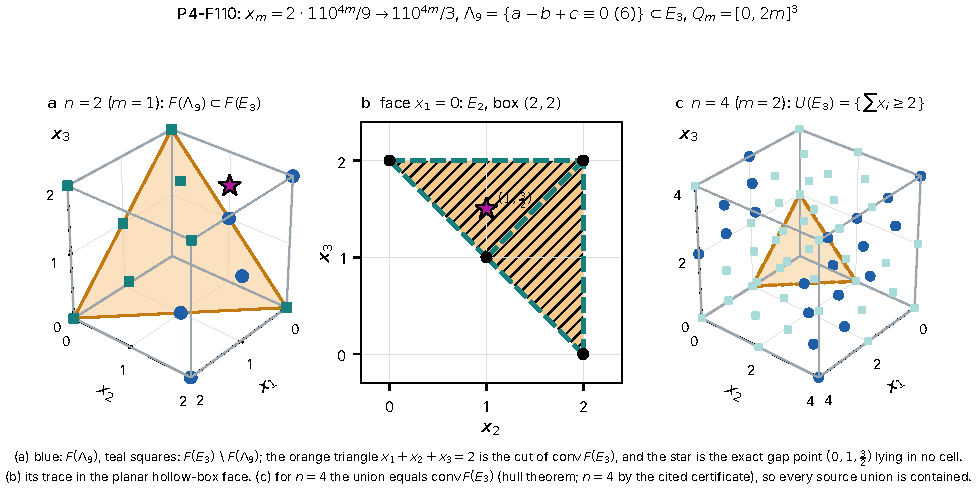
\includegraphics[width=0.98\textwidth]{fig15_f110}
\caption{The coupled family P4-F110 ($x_m=2\cdot110^{4m}/9\to110^{4m}/3$, $\Lambda_9=\{a-b+c\equiv0\ (6)\}\subset E_3$, $Q_m=[0,2m]^3$; \emph{exact computation} for the data, theorem-level for the regime in (c)). (a)~$n=2$ ($m=1$): $F(\Lambda_9,Q_1)$ (5 points) inside $F(E_3,Q_1)$ (13 points); $E_3$ is not hull-covered (\cref{thm:hull}), the point $(0,1,\frac32)$ is in $\conv F(E_3)$ but in no cell of $\Kabs(E_3,Q_1)$. (b)~The face $x_1=0$, where $E_3$ restricts to $E_2$ in the hollow box $(2,2)$ and the gap point appears as $(1,\frac32)$. (c)~$n=4$ ($m=2$): $U(E_3,Q_2)=\{\sum x_i\ge2\}$ by \cref{thm:hull}, with $|F(E_3)|=62$ and $|F(\Lambda_9)|=20$. For $m=1$ containment $U(\Lambda_9)\subseteq U(E_3)$ nevertheless holds (\cref{prop:holes}); for $m\ge2$ it follows from \cref{thm:hull} (see \cref{thm:P4T2}), whose $n=4$ step rests on the certificate of \cref{thm:hull}(3). No claim is drawn from the picture alone.}\label{fig:f110}
\end{figure}

\section{Status, limits, and open problems}\label{sec:open}
\subsection{What is proved and what is not}
\begin{center}\small
\begin{tabular}{@{}p{0.34\textwidth}p{0.17\textwidth}p{0.38\textwidth}@{}}\toprule
result & status & scope\\\midrule
lattice transport (\cref{thm:P2T1}, \cref{prop:E22}) & PROVED & all lattices $\Lambda_b$\\
abstract cell transport (\cref{thm:cell-transport}) & PROVED & all lattices, common box\\
three-stage orbit (\cref{thm:E21}, \cref{cor:threestage}) & PROVED & all $k\ge2$, primes $\equiv2\ (3)$, $2\in\Pcal$\\
planar family (\cref{thm:P2TF1}) & PROVED & $x_h=21^{2h}/5$, $h\ge1$\\
corner cube (\cref{thm:corner}), even-sum (\cref{thm:evensum}) & PROVED & rectangular targets, any $k$; even-sum $k=3$\\
planar monotonicity (\cref{thm:planar}) & PROVED & $k=2$, nested lattices, every box (\cref{lem:T0} proved in \cref{app:lifting})\\
dilation family, no free coordinate (\cref{thm:C1}) & PROVED & $k=3$\\
slab structure and criterion (\cref{thm:slab-i,thm:slab-ii}) & PROVED & split targets, period $k$\\
hull theorem $E_3$ (\cref{thm:hull}) & PROVED mod. cert. & $n\ge4$ even; $n=4$ certificate \cite{HD1P4} cited, replayed in \cref{sec:hard}\\
BCC failure (\cref{prop:C3}) & FINITE-EXACT & $Q=(2,4,2)$\\
census (\cref{prop:census}) & FINITE-EXACT & stated sample, not a theorem\\
specimen counts and Betti numbers (\cref{prop:specimen,prop:topology}) & FINITE-EXACT & the named specimens\\\bottomrule
\end{tabular}
\end{center}
Inherited and cited without reproof: the fibre bijection input (Foundations Vol.~I Thm.~1.2), $D(x)\subseteq D(\Cmap(x))$ (F.T31), the denominator facts behind E2-3, the planar normal form and G12-T8 (GEO-I) and the finite $n=4$ certificate of \cref{thm:hull}. The lifting fact formerly cited as SF is proved in \cref{app:lifting}. Inherited verification of the frozen releases was not re-run; the exact checks of this manuscript are independent re-computations of the worked examples (\texttt{scripts/run\_exact\_checks.py}) and do not constitute external verification.

\subsection{Open problems}
\begin{problem}[which non-split targets preserve $U$]\label{prob:Q1}
Classify the lattices $\Lambda'\subseteq\Z^3$ with no free and no split coordinate for which $U(\Lambda,Q)\subseteq U(\Lambda',Q)$ for \emph{every} $\Lambda\subseteq\Lambda'$ and every box. The census (\cref{prop:census}) shows that $77$ of $84$ sampled targets of index $2$--$6$ show no failure while BCC and six index-$6$ lattices fail; no property of the target that separates the two groups is known (release item P5-Q1).
\end{problem}
\begin{problem}[collective transitions with incomparable lattices]\label{prob:incomp}
For an admissible planar transition with $F\subseteq F'$ but $\Lambda\not\subseteq\Lambda'$ (which occurs, \cref{prop:corpus}), decide whether $U\subseteq U'$. \Cref{thm:planar} does not apply, and \cref{lem:gap} gives containment only in the G12-T8 regime.
\end{problem}
\begin{problem}[dimension $k\ge4$ and exact classification]\label{prob:hd}
Determine the failing cells and the minimal failing boxes for $k\ge4$ and for non-even-sum sources; \cref{thm:corner}(c) bounds the shape of a scaled vertex but does not decide which boxes fail.
\end{problem}
\begin{problem}[embeddedness]\label{prob:emb}
Characterise when $\Kabs(\Lambda,Q)$ is embedded (so that $\Kemb=\Kabs$ and topological statements about $U$ and $\Kabs$ coincide). For the specimen $E_3$, $Q=[0,2]^3$ it is not embedded and $b_2(U)=18\ne b_2(\Kabs)=6$.
\end{problem}
\begin{problem}[tiling lemma; resolved in v0.2]\label{prob:SF}
Remove the dependence of \cref{lem:T0} on the external standard fact SF by a self-contained proof of the covering property of the lower facets. \emph{Resolved:} the proof is given in \cref{app:lifting}. The item is kept so that the numbering of the first version is unchanged.
\end{problem}
\begin{problem}[parameter-family classification and coupled-target theory]\label{prob:T3T4}
The releases name two programmes that were never started: a classification of transport for parameter families beyond P4-F110 (P4-T3), and an essentially three-dimensional theory of coupled-target obstruction (P4-T4). Neither is addressed here. The prior-art search accompanying the releases was limited and is not a novelty clearance; no priority claim is made for any statement of this manuscript.
\end{problem}
The open items recorded at v002 and v003 (\texttt{CW-0493}, \texttt{CW-0495}) comprise: planar containment (resolved by \cref{thm:planar}); the converse of the slab obstruction and the non-existence of ``S1 failures'' (resolved by \cref{cor:S3}); preservation for targets without a free coordinate (resolved negatively by \cref{thm:C1}); and P4-T3, P4-T4 and the prior-art audit (\cref{prob:T3T4}).
\prov{CW-0493}{OPEN(v002)}{OPEN}{OPEN}
\prov{CW-0495}{OPEN(v003)}{OPEN}{OPEN}
\subsection{Conclusion}
Transport of occurrence geometry has three distinct levels. Vertices are transported by the lattice inclusion alone. Cells of the abstract complex are transported exactly when their vertices lie in the target fibre and their generators remain Graver; this can fail for every cell of positive dimension at once. The realised union is transported in the plane for every lattice inclusion and every box, because a cell that touches both axes has its geometry forced by the arithmetic of the axis orders; in dimension three the same inclusion can fail in infinite families, the failure is carried by cells touching all three coordinate planes, and for targets that split along one coordinate the failure is decided exactly by a planar condition on the part of the cell below height $k$. What remains unknown is the full classification in dimension three for non-split targets and the behaviour beyond dimension three.

\clearpage
\phantomsection\addcontentsline{toc}{section}{References}
\begin{thebibliography}{99}\small\raggedright
\bibitem{FoundI} UNNS Substrate programme, \emph{Mathematical Foundations of the UNNS Substrate, Volume~I: Generative Arithmetic and Structural Reachability} (Theorem~1.2, the occurrence set). Source: \texttt{ukbbi/UNNS}, commit \texttt{9a021346b2b3d964523440d2737b9d0c4ddbb3e5}, \texttt{projects/UNNS\_MATH\_FOUNDATIONS/Manuscript}. \url{https://github.com/ukbbi/UNNS/tree/9a021346b2b3d964523440d2737b9d0c4ddbb3e5/projects/UNNS_MATH_FOUNDATIONS/Manuscript}
\bibitem{FoundII} UNNS Substrate programme, \emph{Mathematical Foundations of the UNNS Substrate, Volume~II: Collective Dynamics, Prime Rigidity, and Effective Predictability} (Theorem~1.3 = F.T31, $D(x)\subseteq D(\Cmap(x))$). Same commit and path as~\cite{FoundI}.
\bibitem{RefColl} Foundations reference collection v001 (SELECT-I/II, FIELD-I v001--v012; frozen), \texttt{ukbbi/UNNS}, commit \texttt{bb8b12d753c600c597feb00df17fe139c7cc65fa} (23 Oct.\ 2026), \texttt{projects/UNNS\_MATH\_FOUNDATIONS/sources}. \url{https://github.com/ukbbi/UNNS/tree/bb8b12d753c600c597feb00df17fe139c7cc65fa/projects/UNNS_MATH_FOUNDATIONS/sources}
\bibitem{GEOI} GEO-I releases v001--v012 (planar normal form: v004 S1; planar stabilisation theorem G12-T8: v012). \texttt{ukbbi/UNNS}, commit \texttt{9a021346b2b3d964523440d2737b9d0c4ddbb3e5}, tree \texttt{projects/UNNS\_Higher-Dimensional Geometry}. \url{https://github.com/ukbbi/UNNS/tree/9a021346b2b3d964523440d2737b9d0c4ddbb3e5/projects/UNNS_Higher-Dimensional%20Geometry}
\bibitem{HD1} GEO-HD-1 research collection, snapshot \texttt{a88f31487f3b05c9db297dcd1192d56eea2b0c7d} (the pin named in the programme specification; not independently verified in this work). The source releases of the records of this manuscript, with the SHA-256 of the release archives as recorded in the programme: 
\begin{itemize}[leftmargin=1.4em,itemsep=1pt,topsep=2pt]\footnotesize
\item\label{bib:P1}\texttt{GEO\_HD\_E2\_P1\_v001.zip} \texttt{2463492df1c829c5013ffa2838c9b710f7db20fe172bad80d62c0dd2798f819b} (E2-1..E2-11);
\item\texttt{GEO\_HD\_E2\_P2\_v001.zip} \texttt{5680ab6c0b1c27bd56296ef7ada2924c6db9da695221dc7a4e1ebe2c1c9cd847} (P2-series);
\item\texttt{GEO\_HD\_E2\_P3\_v001.zip} \texttt{7709f4f7bcf206c204634fb5b88ad69e70bef55ed910f5b28ef50f25165dd0f9} (P3-series);
\item\texttt{GEO\_HD\_E2\_P4\_v001.zip} \texttt{6e7190bc03c4f04c9ae032d323ab988816b1214ef3a71530d6ce450244fb7fa6} (P4-series; contains the certificate of \cref{thm:hull}, see~\cite{HD1P4});
\item\texttt{GEO\_HD\_E2\_P4\_v002.zip}, \texttt{\_v003.zip}, \texttt{\_v004.zip}, \texttt{\_v005.zip} (later P4 releases; P5-series in \texttt{v005}) and \texttt{GEO\_HD\_E2\_P4\_v005\_ERRATA\_E1.zip} \texttt{f41a353b71e57bc6df3a7f5858642aea4ff71aa6078ecebbb3e2a6704de6f8b3} (erratum E1, \cref{rem:E1}).
\end{itemize}
\bibitem{HD1P4} Exact finite certificate used in \cref{thm:hull}, $n=4$: file \texttt{results/P4\_CERTIFICATES.json}, key \texttt{n4\_target\_hull\_cover} of the release \texttt{GEO\_HD\_E2\_P4\_v001} (the file is byte-identical in \texttt{v001}--\texttt{v004}; SHA-256 \texttt{5dd01aa86d878bdd53ba31bce71f2a6fba9aa33ce965a53c04b30e0de2682002}, 808\,345 bytes), replayed by shard \texttt{S4} of the release's \texttt{RUN\_VERIFY.py}. See \cref{sec:hard} for its logical role and for the independent replay of this manuscript.
\bibitem{Graver1975} J.~E. Graver, On the foundations of linear and integer linear programming~I, \emph{Math.\ Programming} \textbf{9} (1975), 207--226.
\bibitem{Sturmfels1996} B.~Sturmfels, \emph{Gr\"obner Bases and Convex Polytopes}, University Lecture Series~8, American Mathematical Society, 1996.
\bibitem{DLHK2013} J.~A. De~Loera, R.~Hemmecke, M.~K\"oppe, \emph{Algebraic and Geometric Ideas in the Theory of Discrete Optimization}, MOS--SIAM Series on Optimization~14, SIAM, 2013.
\bibitem{Ziegler1995} G.~M. Ziegler, \emph{Lectures on Polytopes}, Graduate Texts in Mathematics~152, Springer, 1995 (zonotopes, subdivisions and liftings).
\bibitem{DLRS2010} J.~A. De~Loera, J.~Rambau, F.~Santos, \emph{Triangulations: Structures for Algorithms and Applications}, Algorithms and Computation in Mathematics~25, Springer, 2010 (regular subdivisions induced by liftings).
\bibitem{RGZ1994} J.~Richter-Gebert, G.~M. Ziegler, Zonotopal tilings and the Bohne--Dress theorem, in: \emph{Jerusalem Combinatorics '93}, Contemporary Mathematics~178, American Mathematical Society, 1994, 211--232.
\bibitem{HRS2000} B.~Huber, J.~Rambau, F.~Santos, The Cayley trick, lifting subdivisions and the Bohne--Dress theorem on zonotopal tilings, \emph{J.\ Eur.\ Math.\ Soc.} \textbf{2} (2000), 179--198, \texttt{doi:10.1007/s100970050003}.
\bibitem{BLSWZ1999} A.~Bj\"orner, M.~Las~Vergnas, B.~Sturmfels, N.~White, G.~M. Ziegler, \emph{Oriented Matroids}, 2nd ed., Encyclopedia of Mathematics and its Applications~46, Cambridge University Press, 1999 (zonotopal tilings).
\bibitem{Bohne1992} J.~Bohne, \emph{Eine kombinatorische Analyse zonotopaler Raumaufteilungen}, Dissertation, Universit\"at Bielefeld, 1992 (original source of the Bohne--Dress correspondence).
\end{thebibliography}
\paragraph{On the references.} UNNS sources are cited at the commits fixed by the programme, all repository access during this work was read-only, and the URLs above follow GitHub's standard pattern; they were not fetched from the environment in which the manuscript was prepared. The external literature is cited by author, title and publication data; no section numbers of books are quoted, because the arguments of this manuscript that use them are proved in the text (\cref{app:lifting}) or are standard facts of the theory of Graver bases and zonotopes.

\appendix
\section{Theorem map to the crosswalk}\label{app:map}
Every source record allocated to this manuscript (57 rows of the HD-1B line) with its crosswalk row, original theorem identifier, status preserved from the source, proof treatment in this manuscript, and location. Treatments: FULL = full proof here; ADAPTED = proof adapted from the source with its inherited inputs cited; CITED = inherited result cited under its hypotheses; EXAMPLE = used as a worked example or counterexample; FINITE = finite-exact evidence only; OPEN = unresolved; EXCLUDED = not needed (reason in the allocation table).
\begin{center}\scriptsize
\begin{tabular}{@{}llllll@{}}\toprule
CW row & source id & status & treatment & section & number\\\midrule
\texttt{CW-0456} & \texttt{E2-1} & PROVED & FULL & 4 & 4.5\\
\texttt{CW-0457} & \texttt{E2-2} & PROVED & FULL & 3 & 3.1\\
\texttt{CW-0458} & \texttt{E2-3} & PROVED & ADAPTED & 3 & 3.5\\
\texttt{CW-0459} & \texttt{E2-4} & PROVED & ADAPTED & 3 & 3.5\\
\texttt{CW-0460} & \texttt{E2-5} & PROVED & FULL & 4 & 4.4\\
\texttt{CW-0461} & \texttt{E2-6} & PROVED & FULL & 4 & 4.6\\
\texttt{CW-0462} & \texttt{E2-7} & PROVED & ADAPTED & 5 & 5.5\\
\texttt{CW-0463} & \texttt{E2-8} & PROVED & FULL & 6 & 6.1\\
\texttt{CW-0464} & \texttt{E2-10} & FINITE-EXACT & FINITE & 4 & 4.7\\
\texttt{CW-0464} & \texttt{E2-10} & FINITE-EXACT & FINITE & 6 & 6.2\\
\texttt{CW-0465} & \texttt{E2-11} & COUNTEREXAMPLE & EXAMPLE & 6 & 6.4\\
\texttt{CW-0466} & \texttt{P2-L1} & PROVED & FULL & 4 & 4.1\\
\texttt{CW-0467} & \texttt{P2-T1} & PROVED & FULL & 3 & 3.2\\
\texttt{CW-0467} & \texttt{P2-T1} & PROVED & FULL & 3 & 3.3\\
\texttt{CW-0468} & \texttt{P2-L2} & PROVED & FULL & 3 & 3.4\\
\texttt{CW-0469} & \texttt{P2-T2} & PROVED & FULL & 4 & 4.2\\
\texttt{CW-0470} & \texttt{P2-T3} & PROVED & FULL & 4 & 4.3\\
\texttt{CW-0471} & \texttt{P2-TF1} & PROVED & FULL & 4 & 4.8\\
\texttt{CW-0472} & \texttt{P2-D} & FINITE-EXACT & FINITE & 3 & 3.6\\
\texttt{CW-0473} & \texttt{CP2} & OPEN & EXCLUDED & 7 & 7.7\\
\texttt{CW-0474} & \texttt{P2-G} & FINITE-EXACT & FINITE & 6 & 6.3\\
\texttt{CW-0475} & \texttt{E2-P2-V} & PROVED & EXAMPLE & 6 & 6.4\\
\texttt{CW-0476} & \texttt{P3-T0} & PROVED & FULL & 5 & 5.1\\
\texttt{CW-0477} & \texttt{P3-L1} & PROVED & CITED & 7 & 7.7\\
\texttt{CW-0478} & \texttt{P3-C1} & PROVED & CITED & 7 & 7.7\\
\texttt{CW-0479} & \texttt{P3-T3} & PROVED & FULL & 5 & 5.2\\
\texttt{CW-0480} & \texttt{P3-T3(h)} & PROVED & FULL & 5 & 5.4\\
\texttt{CW-0481} & \texttt{P3-T4} & PROVED & EXCLUDED & 5 & 5.6\\
\texttt{CW-0482} & \texttt{CP3-A} & OPEN & EXCLUDED & 7 & 7.7\\
\texttt{CW-0483} & \texttt{P4-A} & PROVED & FULL & 10 & 10.2\\
\texttt{CW-0484} & \texttt{P4-L} & PROVED & FULL & 10 & 10.2\\
\texttt{CW-0485} & \texttt{P4-T1} & PROVED & ADAPTED & 10 & 10.3\\
\texttt{CW-0486} & \texttt{P4-T2} & PROVED-SCOPED & ADAPTED & 10 & 10.4\\
\texttt{CW-0487} & \texttt{P4-C1 (v001)} & CORRECTED & EXCLUDED & 10 & 10.5\\
\texttt{CW-0488} & \texttt{P4-O1} & FINITE-EXACT & FINITE & 10 & 10.6\\
\texttt{CW-0489} & \texttt{P4-C1} & PROVED & FULL & 10 & 10.5\\
\texttt{CW-0490} & \texttt{P4-Z1} & PROVED & FULL & 7 & 7.3\\
\texttt{CW-0491} & \texttt{P4-Z1.a} & PROVED & FULL & 7 & 7.3\\
\texttt{CW-0492} & \texttt{P4-S1} & PROVED & FULL & 9 & 9.2\\
\texttt{CW-0493} & \texttt{OPEN(v002)} & OPEN & OPEN & 11 & 11.6\\
\texttt{CW-0494} & \texttt{P4-S2} & PROVED & ADAPTED & 9 & 9.2\\
\texttt{CW-0495} & \texttt{OPEN(v003)} & OPEN & OPEN & 11 & 11.6\\
\texttt{CW-0496} & \texttt{P4-Z2} & PROVED & FULL & 7 & 7.3\\
\texttt{CW-0497} & \texttt{P4-P1} & PROVED & FULL & 7 & 7.5\\
\texttt{CW-0498} & \texttt{P4-S3} & PROVED & ADAPTED & 9 & 9.5\\
\texttt{CW-0499} & \texttt{E2P4v5-L1} & PROVED & FULL & 7 & 7.1\\
\texttt{CW-0500} & \texttt{E2P4v5-T0} & PROVED & ADAPTED & 7 & 7.2\\
\texttt{CW-0501} & \texttt{E2P4v5-Z} & PROVED & FULL & 7 & 7.3\\
\texttt{CW-0502} & \texttt{E2P4v5-LG} & PROVED & FULL & 7 & 7.4\\
\texttt{CW-0503} & \texttt{E2P4v5-H1} & PROVED & FULL & 10 & 10.1\\
\texttt{CW-0504} & \texttt{P5-P1} & PROVED & FULL & 7 & 7.5\\
\texttt{CW-0505} & \texttt{P5-P1.a} & PROVED & FULL & 7 & 7.8\\
\texttt{CW-0506} & \texttt{P5-F1} & PROVED & FULL & 8 & 8.6\\
\texttt{CW-0507} & \texttt{P5-D1} & PROVED & FULL & 8 & 8.1\\
\texttt{CW-0508} & \texttt{P5-C1} & PROVED & FULL & 8 & 8.2\\
\texttt{CW-0509} & \texttt{P5-C2} & PROVED & FULL & 8 & 8.3\\
\texttt{CW-0510} & \texttt{P5-C3} & FINITE-EXACT & FINITE & 8 & 8.5\\
\texttt{CW-0511} & \texttt{P5-S4} & PROVED & FULL & 9 & 9.1\\
\texttt{CW-0511} & \texttt{P5-S4(ii)'} & PROVED & FULL & 9 & 9.3\\
\texttt{CW-0512} & \texttt{census} & FINITE-EXACT & FINITE & 8 & 8.7\\
\bottomrule\end{tabular}
\end{center}


\section{Proof of the lifting lemma used in \texorpdfstring{\cref{lem:T0}}{Lemma 7.2}}\label{app:lifting}
The tiling lemma (\cref{lem:T0}) uses the standard statement that the lower facets of a lifted polytope project onto its shadow with disjoint interiors (the regular subdivision induced by a lifting, \cite{Ziegler1995,DLRS2010}; the construction behind the Bohne--Dress correspondence \cite{Bohne1992,RGZ1994,HRS2000,BLSWZ1999}). For completeness the argument is given here.

Let $\pi:\R^{d+1}\to\R^d$ forget the last coordinate and let $\tilde P\subset\R^{d+1}$ be a polytope with non-empty interior, $P=\pi(\tilde P)$. A face of $\tilde P$ is \emph{lower} if it is the set of maximisers of some linear functional $\nu=(\nu',\nu_{d+1})$ with $\nu_{d+1}<0$ on $\tilde P$; a lower facet is a lower face of dimension $d$.
\begin{lemma}[lifting]\label{lem:lift}
(i) On every lower face $G$ the projection $\pi$ is an affine isomorphism onto $\pi(G)$; (ii) the sets $\pi(F)$, $F$ a lower facet, cover $P$; (iii) the interiors of $\pi(F)$ and $\pi(F')$ are disjoint for distinct lower facets $F\ne F'$.
\end{lemma}
\begin{proof}
Put $h(x)=\min\{t:(x,t)\in\tilde P\}$ for $x\in P$.

(i) Let $G$ be the set of maximisers of $\nu$ with $\nu_{d+1}<0$ and $(x,t)\in G$. If $(x,t')\in\tilde P$ with $t'<t$, then $\nu\cdot(x,t')-\nu\cdot(x,t)=\nu_{d+1}(t'-t)>0$, contradicting maximality; hence $t=h(x)$. So $G\subseteq\{(x,h(x))\}$ and $\pi|_G$ is injective, and an injective affine map on a polytope is an affine isomorphism onto its image; in particular $\dim\pi(G)=\dim G\le d$.

(ii) The set $\pi(\mathrm{int}\,\tilde P)$ is open (since $\pi$ is an open map), convex, and dense in $P$; for a convex set $C$ with $\overline C=P$ one has $\mathrm{int}\,P=\mathrm{int}\,C$, so $\pi(\mathrm{int}\,\tilde P)=\mathrm{int}\,P$. Let $x\in\mathrm{int}\,P$ and $y=(x,h(x))$. The fibre $\tilde P\cap(\{x\}\times\R)$ contains a point $(x,t_0)$ of $\mathrm{int}\,\tilde P$, and $y\in\partial\tilde P$ by minimality of $h(x)$. Let $\nu$ be a supporting functional at $y$, $G_\nu=\{z\in\tilde P:\nu\cdot z=\nu\cdot y\}$. Since $(x,t)\in\tilde P$ for $t\ge h(x)$ near $t_0$ we have $\nu_{d+1}\le0$; and $\nu_{d+1}=0$ would give $\nu\cdot(x,t_0)=\nu\cdot y$, i.e.\ an interior point of $\tilde P$ on a supporting hyperplane, which is impossible. Hence $\nu_{d+1}<0$, so $y$ lies in a lower face $G_\nu$ and $x\in\pi(G_\nu)$. Thus $\mathrm{int}\,P\subseteq\bigcup\pi(G)$ over lower faces $G$. The lower faces of dimension $<d$ project (by (i)) to finitely many polytopes of dimension $<d$, a closed set with empty interior; a lower face of dimension $d$ is a lower facet. So the union of $\pi(F)$ over lower facets is a closed set that contains a dense subset of $\mathrm{int}\,P$, hence contains $\mathrm{int}\,P$ and, being closed, $P=\overline{\mathrm{int}\,P}$.

(iii) Let $F\ne F'$ be lower facets and $x$ an interior point of both $\pi(F)$ and $\pi(F')$. By (i) the points of $F,F'$ above $x$ are both equal to $y=(x,h(x))$, so $y\in F\cap F'$; as $\pi|_F$, $\pi|_{F'}$ are affine isomorphisms onto $d$-dimensional sets and $x$ is interior to the images, $y$ lies in the relative interior of both $F$ and $F'$. But a point of a polytope lies in the relative interior of exactly one face, so $F=F'$. \qedhere
\end{proof}
\begin{remark}
For the zonotope $\tilde Z=\sum[0,1]\tilde v_i$ of \cref{lem:T0}, full-dimensionality holds because, for $n>d$ and generic heights, some lifted generator is not in the span of the $d$ others of a basis; the lemma then gives that the lower facets $\sum_{i\in A_S}\tilde v_i+Z(\tilde v_S)$ project onto tiles $T_S$ that cover $Z(V)$ with disjoint interiors, which is the claim of \cref{lem:T0}.
\end{remark}

\end{document}
